\chapter{拓扑能带论}

本节要讨论的系统和\autoref{chap:conventional-metal}的哈密顿量基本上是差不多的:系统的基本自由度是某种电子,可以完全使用能带理论刻画它,相互作用可以忽略。
然而,特殊的拓扑性质会让这些系统展现出和普通的金属、绝缘体非常不同的行为。

\section{拓扑绝缘体}

\begin{back}{绝热演化}{adiabatic}
    哈密顿量变化,系统的基态和激发态也会随之变化。哈密顿量的局域、连续的变化\emph{不能}让基态和激发态遍历所有的可能。
    例如,基态和激发态之间是否存在能隙这件事在哈密顿量的连续局域变化下是不会变的。
    这些诸如能隙有无之类的东西可以看成拓扑不变量,据此我们可以对哈密顿量做拓扑分类。
\end{back}

绝缘体中化学势位于两条能带中间,因此有明确的、彼此之间不连续的价带和导带,换而言之,载流子存在能隙(见\autoref{sec:conductor-classification})。
另一方面,导体中载流子不存在能隙。
单电子能谱是否存在能隙也决定了\emph{电子态}具有或者不具有能隙,因为多电子态能够发生的最小偏移就是多一个或者少一个电子。

既然连续地、局域地调节哈密顿量不会改变能隙的有无,我们可以据此定义一个拓扑等价类。
% TODO:平庸芯能带
所有的传统绝缘体(就是\autoref{chap:conventional-metal}中出现的那些)都可以归入一类,这个类别中也包括真空,因为真空中的电子同样可以认为有一个价带(电子)和一个满带(正电子),两者之间存在能隙。

\section{整数量子霍尔效应}

具有能隙的电子态同样可以因为拓扑而有非平凡的行为,典型的例子是\concept{整数量子霍尔效应}。

\subsection{整数电导平台}

实际的体系中有杂质,因此朗道能级会出现展宽,并且两个朗道能级之间的态基本上是局域化态(朗道能级中的态则比较舒展)。
换而言之,朗道能级附近的电子可以自由移动,贡献电导,而两个朗道能级之间的电子高度定域,并不贡献电导。
因此,随着电子数上升,在填充延展态时电导线性上升,而在填充定域态时电导没有变化。这就形成了\concept{电导平台}。
相应的,平台处的霍尔电导为
\[
    \sigma_\text{H} = n \frac{e^2}{h}, \quad n = 0, 1, 2, \ldots,
\]
称为\concept{整数霍尔效应}。
总之,要形成量子霍尔效应,对电导有贡献的能级必须有能隙。

这就造成了一个非常矛盾的情况:要观察到电导平台,体系必须比较“脏”,这样才能够有明确的定域态,从而形成平台;但实际上,在体系很脏时朗道能级附近的延展态也被破坏了,因此太脏的体系展现不出太多平台。
因此明显的量子霍尔效应需要体系有些脏但又不太脏。

“对电导有贡献的能级必须有能隙”还产生了一个问题:既然有能隙,那么在化学势位于能隙之中时如何形成显著的电流?
唯一的可能是,体态有能隙,但边界态没有能隙,从而边界态导电。(这还意味着一件事:体态有能隙说明体态内部的关联长度有限,因此边界态和体态相对独立)
可以从一个经典图像看到这一点:在体态中电子可以不停做圆周运动,而在边界附近电子做完半个圆周运动后被反弹,而又往前做半个圆周运动。
因此,可以形成绕着整个边界运行的(手性的)电流。边界态上如果有杂质,电子可以潜到体态中,绕过杂质,形成一个新的边界态。因此边界态上的电流是无损耗的。

关于为什么霍尔电导取非常简洁的形式(通常的电导涉及关于材料的复杂性质),\concept{Laughlin论证}给出了一个解释。
设有一个半径为$L$的圆柱体,其体态有能隙而边界态导电。
沿着它的轴向加入一个磁场,总磁通量为$\Phi$。让$\Phi$缓慢地发生变化,从零变化到$\frac{h c}{e}$,则$\Phi$变化前后圆柱体均处于同样的状态,因为绕着大小为$\frac{h c}{e}$的磁通量转一圈什么也不会发生。
磁通量的变化会导致一个电场,在边界上,我们有
\[
    2 \pi L E = - \frac{1}{c} \dv{\Phi}{t},
\]
从而
\[
    E(t) = \frac{1}{2\pi L c} \dv{\Phi}{t}.
\]
边界上的电场方向垂直轴向,从而产生一个平行于轴向的霍尔电流
\[
    I = 2 \pi L j = 2 \pi L \sigma_\text{H} E = \frac{\sigma_\text{H}}{c} \dv{\Phi}{t}.
\]
这个电流造成的电荷量变化为
\[
    \Delta Q = \int \dd{t} I = \frac{\sigma_\text{H}}{c} \Delta \Phi = \sigma_\text{H} \frac{h}{e},
\]
而由于电荷由电子携带,有
\[
    \Delta Q = me, \quad m = 0, 1, 2, \ldots,
\]
于是
\[
    \sigma_\text{H} = m \frac{e^2}{h}, \quad m = 0, 1, 2, \ldots.
\]
这就是整数阶量子霍尔效应的来源:它和体系的结构完全无关,只要体系体态有能隙,就能够得出存在整数霍尔效应的结论。

\subsection{$1/m$型分数量子霍尔效应}

既然Laughlin论证只能够得到整数量子霍尔效应,我们要问,分数量子霍尔效应是怎么产生的。
显然,唯一的可能是,电子之间的相互作用产生了分数阶能级。
本节讨论
\[
    \nu = \frac{1}{m}, \quad m = 1, 3, 5, \ldots
\]
型的分数量子霍尔效应,这是最简单的情况。

Laughlin通过其天才的创造,一步到位地给出了能产生分数霍尔效应的波函数:
\begin{equation}
    \Phi(z_1, \ldots, z_N) = \prod_{i < j} (z_{\vb*{i}} - z_j)^{m} \ee^{- \sum_{\vb*{i}} \abs*{z_{\vb*{i}}}^2 / 4 l_0^2}, \quad m = 1, 3, 5, \ldots.
\end{equation}
容易验证以上波函数满足交换反对称性;当$z_{\vb*{i}}$趋于$z_j$时波函数趋于零,这是库伦排斥的结果。

\chapter{自旋系统中的拓扑序}

本章列出一些展现了拓扑序的自旋系统。

\section{Toric-code模型}

\subsection{Toric-code哈密顿量与解析解}

Kitaev最早提出了一种模型,作为一种可能的量子计算纠错编码,他发现这个模型放在一个环面上可以有非常有趣的结果。
然而,事后发现这个模型实际上展现出了一个拓扑序。

\begin{figure}
    \centering
    \subfigure[Toric-code模型的希尔伯特空间的一组基底由这样的态构成:每条边上都或是有确定的$\sigma^z$或是有确定的$\sigma^x$]{
        \documentclass[hyperref, UTF8, a4paper]{ctexart}

\usepackage{geometry}
\usepackage{titling}
\usepackage{titlesec}
\usepackage{paralist}
\usepackage{footnote}
\usepackage{enumerate}
\usepackage{amsmath, amssymb, amsthm}
\usepackage{bbm}
\usepackage{cite}
\usepackage{graphicx}
\usepackage{subfigure}
\usepackage{physics}
\usepackage{tikz}
\usepackage{autobreak}
\usepackage[ruled, vlined, linesnumbered, noend]{algorithm2e}
\usepackage[colorlinks, linkcolor=black, anchorcolor=black, citecolor=black]{hyperref}
\usepackage{prettyref}

% Page style
\geometry{left=3.18cm,right=3.18cm,top=2.54cm,bottom=2.54cm}
\titlespacing{\paragraph}{0pt}{1pt}{10pt}[20pt]
\setlength{\droptitle}{-5em}
\preauthor{\vspace{-10pt}\begin{center}}
\postauthor{\par\end{center}}

% Math operators
\DeclareMathOperator{\timeorder}{T}
\DeclareMathOperator{\diag}{diag}
\DeclareMathOperator{\legpoly}{P}
\DeclareMathOperator{\primevalue}{P}
\DeclareMathOperator{\sgn}{sgn}
\newcommand*{\ii}{\mathrm{i}}
\newcommand*{\ee}{\mathrm{e}}
\newcommand*{\const}{\mathrm{const}}
\newcommand*{\comment}{\paragraph{注记}}
\newcommand*{\suchthat}{\quad \text{s.t.} \quad}
\newcommand*{\argmin}{\arg\min}
\newcommand*{\argmax}{\arg\max}
\newcommand*{\normalorder}[1]{: #1 :}
\newcommand*{\pair}[1]{\langle #1 \rangle}
\newcommand*{\fd}[1]{\mathcal{D} #1}
\DeclareMathOperator{\bigO}{\mathcal{O}}

% prettyref setting
\newrefformat{sec}{第\ref{#1}节}
\newrefformat{note}{注\ref{#1}}
\newrefformat{fig}{图\ref{#1}}
\newrefformat{alg}{算法\ref{#1}}
\renewcommand{\autoref}{\prettyref}

% TikZ setting
\usetikzlibrary{arrows,shapes,positioning}
\usetikzlibrary{arrows.meta}
\usetikzlibrary{decorations.markings}
\tikzstyle arrowstyle=[scale=1]
\tikzstyle directed=[postaction={decorate,decoration={markings,
    mark=at position .5 with {\arrow[arrowstyle]{stealth}}}}]
\tikzstyle ray=[directed, thick]
\tikzstyle dot=[anchor=base,fill,circle,inner sep=1pt]

% Algorithm setting
\renewcommand{\algorithmcfname}{算法}
% Python-style code
\SetKwIF{If}{ElseIf}{Else}{if}{:}{elif:}{else:}{}
\SetKwFor{For}{for}{:}{}
\SetKwFor{While}{while}{:}{}
\SetKwInput{KwData}{输入}
\SetKwInput{KwResult}{输出}
\SetArgSty{textnormal}

\renewcommand{\emph}[1]{\textbf{#1}}
\newcommand*{\concept}[1]{\underline{\textbf{#1}}}
\newcommand*{\Ztwo}{$\mathbb{Z}_2$}

\title{常见格点模型}
\author{吴何友}

\begin{document}

\maketitle

\section{相互作用体系}

\subsection{Hubbard模型}

\concept{Hubbard模型}是一种常见的强关联电子模型,它是一个定义在点阵上的模型,以下我们照惯例用$i, j$等表示格点坐标。
不包含化学势的哈密顿量为
\begin{equation}
    \hat{H} = \underbrace{-t \sum_{\pair{i, j}, \sigma} \hat{c}_{i\sigma}^\dagger \hat{c}_{j\sigma} + \text{h.c.}}_{\hat{H}_0} + \underbrace{U \sum_i \hat{n}_{i \uparrow} \hat{n}_{i \downarrow}}_{\hat{H}_\text{I}}.
\end{equation}
或者,为了后面蒙特卡洛模拟的方便,重新定义化学势,也可以有
\begin{equation}
    \hat{H} = -t \sum_{\pair{i, j}, \sigma} \hat{c}_{i\sigma}^\dagger \hat{c}_{j\sigma} + \text{h.c.} 
    + U \sum_i \left(\hat{n}_{i\uparrow} - \frac{1}{2}\right) \left(\hat{n}_{i\downarrow} - \frac{1}{2}\right).
\end{equation}

\subsubsection{Hubbard模型的量子蒙特卡洛模拟}

\subsection{Trotter分解和辅助场引入}

下面我们尝试对Hubbard模型做Trotter分解。设虚时间间隔为$\Delta\tau$,总共有$m$个虚时间点,$\tau=m\Delta \tau$。
对Hubbard模型,有一种特殊的分解方法:
\begin{equation}
    \ee^{-\Delta \tau \hat{H}_\text{I}} = \gamma \sum_{s_1, s_2, \ldots, s_N = \pm 1} \ee^{\alpha \sum_i s_i (\hat{n}_{i\uparrow} - \hat{n}_{i \downarrow})}, 
    \quad \gamma = \frac{1}{2^N} \ee^{\Delta \tau U N / 4}, \quad \cosh(\alpha) = \ee^{\Delta \tau U / 2},
\end{equation}
可以看到$\gamma$是一个和辅助场$\{s_i\}$(照惯例我们下面记它的时间线为$\vb{s}$)无关的量,考虑到配分函数的常数因子无关紧要,略去此因子,则配分函数为
\[
    \begin{aligned}
        Z &= \trace \prod_{n=1}^m \sum_{\vb{s}_{n}} \ee^{\alpha \sum_i s_i (\hat{n}_{i\uparrow} - \hat{n}_{i \downarrow})} \ee^{\Delta \tau t \sum_{\pair{i, j}, \sigma} \hat{c}_{i\sigma}^\dagger \hat{c}_{j\sigma} + \text{h.c.}} \\
        &= \sum_{\vb{s}} \prod_{n=1}^m \ee^{\alpha \hat{c}^\dagger_{\uparrow} \diag{\vb{s}_n} \hat{c}_{\uparrow}} \ee^{- \alpha \hat{c}^\dagger_{\downarrow} \diag{\vb{s}_n} \hat{c}_{\downarrow}} \ee^{- \Delta \tau \hat{c}_\uparrow^\dagger \vb{T} \hat{c}_\uparrow} \ee^{- \Delta \tau \hat{c}_\downarrow^\dagger \vb{T} \hat{c}_\downarrow},
    \end{aligned}
\]
其中我们指定$\vb{T}$是动能部分$\hat{H}_0$在单粒子表象下的系数矩阵,即
\begin{equation}
    T_{ij} = \begin{cases}
        -t, \quad &\pair{i, j}, \\
        0, \quad &\text{otherwise}.
    \end{cases}
\end{equation}
应用公式
\begin{equation}
    \trace(\ee^{- \sum_{i, j} \hat{c}_i^\dagger A_{ij} \hat{c}_j} \ee^{- \sum_{i, j} \hat{c}_i^\dagger B_{ij} \hat{c}_j} \cdots) = \det(1 + \ee^{- \vb{A}}\ee^{- \vb{B}} \cdots),
    \label{eq:trace-to-det}
\end{equation}
我们积掉费米子自由度,得到
\[
    Z = \sum_{\vb{s}} \det(1 + \prod_{n=1}^m \exp(\alpha \diag{\vb{s}_n \oplus (-\vb{s}_n)}) \exp( -\Delta \tau \pmqty{\dmat{\vb{T}, \vb{T}}})).
\]
上式中出现了矩阵拼接,因为电子的量子数同时包括位置和自旋,因此需要$2N \times 2N$的矩阵(在$2N$维中,前$N$维对应自旋向上的态,后$N$维对应自旋向下的态)。
然而,Hubbard模型的自选旋转不变性意味着以上矩阵是分块对角的,从而可以拆分开来,得到下式:
\begin{equation}
    Z = \det(1 + \prod_{\sigma=\uparrow, \downarrow} \prod_{n=1}^m \vb{B}_{\vb{s}}^\sigma(\tau) ),
\end{equation}
其中
\begin{equation}
    \vb{B}^\uparrow_{\vb{s}}(\tau) = \ee^{\alpha \diag \vb{s}_n} \ee^{-\Delta \tau \vb{T}}, \quad \vb{B}^\downarrow_{\vb{s}}(\tau) = \ee^{- \alpha \diag \vb{s}_n} \ee^{-\Delta \tau \vb{T}}.
\end{equation}
所有$\vb{B}_{\sigma}$都是一个$N \times N$矩阵,而不是$2N \times 2N$的矩阵。

\section{磁场}

将电子和一个满足库伦规范的磁矢势$\vb*{A}$耦合,那么会出现动量的一个修正,这个修在在波函数上引入如下的相位变化:
\begin{equation}
    \theta = \int \dd{\vb*{l}} \cdot \vb*{A}.
\end{equation}
在格点模型中,电子仅仅出现在格点上。我们知道紧束缚模型的哈密顿量(即跃迁项)实际上就是动能,因此加入磁场意味着紧束缚模型的$t_{ij}$出现变化,考虑相位变化,则磁场会导致以下修正:
\begin{equation}
    t_{ij} \longrightarrow \ee^{\ii e \int_j^i \dd{\vb*{l}} \cdot \vb*{A} } t_{ij}.
\end{equation}
相应的,设一个格点上的闭合路径为$C$,通过它的磁通量为$\Phi$,则
\begin{equation}
    \ee^{\ii \Phi} = \prod_{C} t_{ij}.
\end{equation}

\end{document}
    }
    \subfigure[$A$激发定义在格点上,上图是一个$A$激发的例子]{
        

\tikzset{every picture/.style={line width=0.75pt}} %set default line width to 0.75pt        

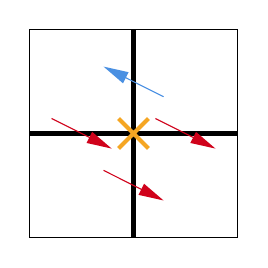
\begin{tikzpicture}[x=0.75pt,y=0.75pt,yscale=-1,xscale=1]
%uncomment if require: \path (0,300); %set diagram left start at 0, and has height of 300

%Shape: Square [id:dp6654025093743159] 
\draw   (140,67) -- (190,67) -- (190,117) -- (140,117) -- cycle ;
%Shape: Square [id:dp6286524465515233] 
\draw   (190,67) -- (240,67) -- (240,117) -- (190,117) -- cycle ;
%Shape: Square [id:dp6519468109347835] 
\draw   (140,117) -- (190,117) -- (190,167) -- (140,167) -- cycle ;
%Shape: Square [id:dp2265935355822739] 
\draw   (190,117) -- (240,117) -- (240,167) -- (190,167) -- cycle ;
%Straight Lines [id:da21658691245720751] 
\draw [line width=1.5]    (190,67) -- (190,117) ;
%Straight Lines [id:da3177017321913107] 
\draw [line width=1.5]    (140,117) -- (190,117) ;
%Straight Lines [id:da01915738195349781] 
\draw [line width=1.5]    (190,117) -- (190,167) ;
%Straight Lines [id:da717616113838583] 
\draw [line width=1.5]    (190,117) -- (240,117) ;
%Straight Lines [id:da8258680195288246] 
\draw [color={rgb, 255:red, 245; green, 166; blue, 35 }  ,draw opacity=1 ][line width=1.5]    (190,117) ;
\draw [shift={(190,117)}, rotate = 45] [color={rgb, 255:red, 245; green, 166; blue, 35 }  ,draw opacity=1 ][line width=1.5]    (-10.17,0) -- (10.17,0)(0,10.17) -- (0,-10.17)   ;
%Straight Lines [id:da10440190731652677] 
\draw [color={rgb, 255:red, 208; green, 2; blue, 27 }  ,draw opacity=1 ]   (200.54,109.75) -- (227.67,123.35) ;
\draw [shift={(229.46,124.25)}, rotate = 206.63] [fill={rgb, 255:red, 208; green, 2; blue, 27 }  ,fill opacity=1 ][line width=0.08]  [draw opacity=0] (12,-3) -- (0,0) -- (12,3) -- cycle    ;
%Straight Lines [id:da6468653685487751] 
\draw [color={rgb, 255:red, 74; green, 144; blue, 226 }  ,draw opacity=1 ]   (204.46,99.25) -- (177.33,85.65) ;
\draw [shift={(175.54,84.75)}, rotate = 386.63] [fill={rgb, 255:red, 74; green, 144; blue, 226 }  ,fill opacity=1 ][line width=0.08]  [draw opacity=0] (12,-3) -- (0,0) -- (12,3) -- cycle    ;
%Straight Lines [id:da7493786508982636] 
\draw [color={rgb, 255:red, 208; green, 2; blue, 27 }  ,draw opacity=1 ]   (175.54,134.75) -- (202.67,148.35) ;
\draw [shift={(204.46,149.25)}, rotate = 206.63] [fill={rgb, 255:red, 208; green, 2; blue, 27 }  ,fill opacity=1 ][line width=0.08]  [draw opacity=0] (12,-3) -- (0,0) -- (12,3) -- cycle    ;
%Straight Lines [id:da32966501733867193] 
\draw [color={rgb, 255:red, 208; green, 2; blue, 27 }  ,draw opacity=1 ]   (150.54,109.75) -- (177.67,123.35) ;
\draw [shift={(179.46,124.25)}, rotate = 206.63] [fill={rgb, 255:red, 208; green, 2; blue, 27 }  ,fill opacity=1 ][line width=0.08]  [draw opacity=0] (12,-3) -- (0,0) -- (12,3) -- cycle    ;




\end{tikzpicture}
      
    }
    \vfill
    \subfigure[$B$激发定义在正方形方块上,上图是一个$B$激发的例子]{
        

\tikzset{every picture/.style={line width=0.75pt}} %set default line width to 0.75pt        

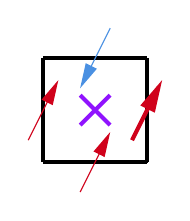
\begin{tikzpicture}[x=0.75pt,y=0.75pt,yscale=-1,xscale=1]
%uncomment if require: \path (0,300); %set diagram left start at 0, and has height of 300

%Shape: Square [id:dp06008287812795965] 
\draw   (192,54) -- (242,54) -- (242,104) -- (192,104) -- cycle ;
%Straight Lines [id:da5345790011660227] 
\draw [line width=1.5]    (192,54) -- (192,104) ;
%Straight Lines [id:da8934908293124699] 
\draw [line width=1.5]    (242,54) -- (242,104) ;
%Straight Lines [id:da6163816696768483] 
\draw [line width=1.5]    (192,54) -- (242,54) ;
%Straight Lines [id:da13968764975578463] 
\draw [line width=1.5]    (192,104) -- (242,104) ;
%Straight Lines [id:da6360739318940407] 
\draw [color={rgb, 255:red, 208; green, 2; blue, 27 }  ,draw opacity=1 ]   (184.75,93.46) -- (198.35,66.33) ;
\draw [shift={(199.25,64.54)}, rotate = 476.63] [fill={rgb, 255:red, 208; green, 2; blue, 27 }  ,fill opacity=1 ][line width=0.08]  [draw opacity=0] (12,-3) -- (0,0) -- (12,3) -- cycle    ;
%Straight Lines [id:da2436020984695373] 
\draw [color={rgb, 255:red, 74; green, 144; blue, 226 }  ,draw opacity=1 ]   (224.25,39.54) -- (210.65,66.67) ;
\draw [shift={(209.75,68.46)}, rotate = 296.63] [fill={rgb, 255:red, 74; green, 144; blue, 226 }  ,fill opacity=1 ][line width=0.08]  [draw opacity=0] (12,-3) -- (0,0) -- (12,3) -- cycle    ;
%Straight Lines [id:da6361964039179109] 
\draw [color={rgb, 255:red, 208; green, 2; blue, 27 }  ,draw opacity=1 ][line width=1.5]    (234.75,93.46) -- (247.46,68.12) ;
\draw [shift={(249.25,64.54)}, rotate = 476.63] [fill={rgb, 255:red, 208; green, 2; blue, 27 }  ,fill opacity=1 ][line width=0.08]  [draw opacity=0] (15.6,-3.9) -- (0,0) -- (15.6,3.9) -- cycle    ;
%Straight Lines [id:da7397146382660318] 
\draw [color={rgb, 255:red, 208; green, 2; blue, 27 }  ,draw opacity=1 ]   (209.75,118.46) -- (223.35,91.33) ;
\draw [shift={(224.25,89.54)}, rotate = 476.63] [fill={rgb, 255:red, 208; green, 2; blue, 27 }  ,fill opacity=1 ][line width=0.08]  [draw opacity=0] (12,-3) -- (0,0) -- (12,3) -- cycle    ;
%Straight Lines [id:da059453193677352134] 
\draw [color={rgb, 255:red, 144; green, 19; blue, 254 }  ,draw opacity=1 ][line width=1.5]    (217,79) ;
\draw [shift={(217,79)}, rotate = 45] [color={rgb, 255:red, 144; green, 19; blue, 254 }  ,draw opacity=1 ][line width=1.5]    (-10.17,0) -- (10.17,0)(0,10.17) -- (0,-10.17)   ;




\end{tikzpicture}
    }
    \subfigure[虽然$\sigma^x$和$\sigma^z$之间有量子涨落,但是$A$和$B$对易,从而系统的能量本征态可以用$A$激发和$B$激发标记;通过数自由度会发现也只需要这两个标记]{
        

\tikzset{every picture/.style={line width=0.75pt}} %set default line width to 0.75pt        

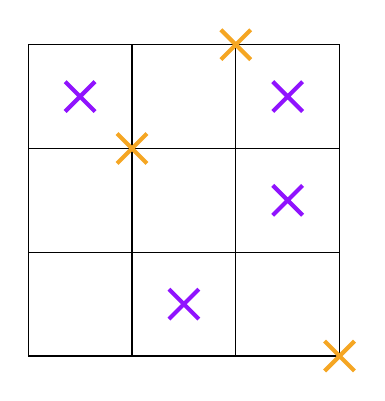
\begin{tikzpicture}[x=0.75pt,y=0.75pt,yscale=-1,xscale=1]
%uncomment if require: \path (0,300); %set diagram left start at 0, and has height of 300

%Shape: Square [id:dp4570817602982631] 
\draw   (100,29) -- (150,29) -- (150,79) -- (100,79) -- cycle ;
%Shape: Square [id:dp2903299358971252] 
\draw   (150,29) -- (200,29) -- (200,79) -- (150,79) -- cycle ;
%Shape: Square [id:dp8410481858286352] 
\draw   (100,79) -- (150,79) -- (150,129) -- (100,129) -- cycle ;
%Shape: Square [id:dp1117017430126368] 
\draw   (150,79) -- (200,79) -- (200,129) -- (150,129) -- cycle ;
%Shape: Square [id:dp9054195019818092] 
\draw   (200,29) -- (250,29) -- (250,79) -- (200,79) -- cycle ;
%Shape: Square [id:dp9918567360750739] 
\draw   (200,79) -- (250,79) -- (250,129) -- (200,129) -- cycle ;
%Shape: Square [id:dp6694249449139529] 
\draw   (100,129) -- (150,129) -- (150,179) -- (100,179) -- cycle ;
%Shape: Square [id:dp6467857772283392] 
\draw   (150,129) -- (200,129) -- (200,179) -- (150,179) -- cycle ;
%Shape: Square [id:dp32240121043282777] 
\draw   (200,129) -- (250,129) -- (250,179) -- (200,179) -- cycle ;
%Straight Lines [id:da5972676544083908] 
\draw [color={rgb, 255:red, 245; green, 166; blue, 35 }  ,draw opacity=1 ][line width=1.5]    (150,79) ;
\draw [shift={(150,79)}, rotate = 45] [color={rgb, 255:red, 245; green, 166; blue, 35 }  ,draw opacity=1 ][line width=1.5]    (-10.17,0) -- (10.17,0)(0,10.17) -- (0,-10.17)   ;
%Straight Lines [id:da06771970628563428] 
\draw [color={rgb, 255:red, 245; green, 166; blue, 35 }  ,draw opacity=1 ][line width=1.5]    (250,179) ;
\draw [shift={(250,179)}, rotate = 45] [color={rgb, 255:red, 245; green, 166; blue, 35 }  ,draw opacity=1 ][line width=1.5]    (-10.17,0) -- (10.17,0)(0,10.17) -- (0,-10.17)   ;
%Straight Lines [id:da1804222983474455] 
\draw [color={rgb, 255:red, 245; green, 166; blue, 35 }  ,draw opacity=1 ][line width=1.5]    (200,29) ;
\draw [shift={(200,29)}, rotate = 45] [color={rgb, 255:red, 245; green, 166; blue, 35 }  ,draw opacity=1 ][line width=1.5]    (-10.17,0) -- (10.17,0)(0,10.17) -- (0,-10.17)   ;
%Straight Lines [id:da7901030413597554] 
\draw [color={rgb, 255:red, 144; green, 19; blue, 254 }  ,draw opacity=1 ][line width=1.5]    (175,154) ;
\draw [shift={(175,154)}, rotate = 45] [color={rgb, 255:red, 144; green, 19; blue, 254 }  ,draw opacity=1 ][line width=1.5]    (-10.17,0) -- (10.17,0)(0,10.17) -- (0,-10.17)   ;
%Straight Lines [id:da37933960521297805] 
\draw [color={rgb, 255:red, 144; green, 19; blue, 254 }  ,draw opacity=1 ][line width=1.5]    (225,104) ;
\draw [shift={(225,104)}, rotate = 45] [color={rgb, 255:red, 144; green, 19; blue, 254 }  ,draw opacity=1 ][line width=1.5]    (-10.17,0) -- (10.17,0)(0,10.17) -- (0,-10.17)   ;
%Straight Lines [id:da13742234427535593] 
\draw [color={rgb, 255:red, 144; green, 19; blue, 254 }  ,draw opacity=1 ][line width=1.5]    (125,54) ;
\draw [shift={(125,54)}, rotate = 45] [color={rgb, 255:red, 144; green, 19; blue, 254 }  ,draw opacity=1 ][line width=1.5]    (-10.17,0) -- (10.17,0)(0,10.17) -- (0,-10.17)   ;
%Straight Lines [id:da5163777331330268] 
\draw [color={rgb, 255:red, 144; green, 19; blue, 254 }  ,draw opacity=1 ][line width=1.5]    (225,54) ;
\draw [shift={(225,54)}, rotate = 45] [color={rgb, 255:red, 144; green, 19; blue, 254 }  ,draw opacity=1 ][line width=1.5]    (-10.17,0) -- (10.17,0)(0,10.17) -- (0,-10.17)   ;




\end{tikzpicture}

    }
    \caption{Toric-code模型的系统构型和元激发}
\end{figure}

考虑一个正方晶格,在每条边(\emph{不是}每个格点!)上放有一个自旋$1/2$自由度。
哈密顿量为
\begin{equation}
    {H} = - \sum_s {A}_s - \sum_p {B}_p,
    \label{eq:toric-code-hamiltonian}
\end{equation}
其中下标$s$表示格点,${A}_s$指的是格点$s$周围的四条边上的$x$方向上的自旋算符的乘积,即
\begin{equation}
    {A}_s = \prod_{\vb*{i} \text{ near } s} {\sigma}_{\vb*{i}}^x,
\end{equation}
而$p$表示格点中的一个最小正方形方块,${B}_p$指的是正方形$p$的四条边上的$z$方向上的自旋算符的乘积,即
\begin{equation}
    {B}_p = \prod_\text{$\vb*{i}$ of $p$} {\sigma}_{\vb*{i}}^z.
\end{equation}

\eqref{eq:toric-code-hamiltonian}是严格可解的。
首先可以验证$\{{A}_s\}$和$\{{B}_p\}$构成一组对易稳定子(即平方为1的一组彼此对易的厄米算符),这样就有
\begin{equation}
    \comm*{{A}_s}{{H}} = \comm*{{B}_p}{{H}} = 0.
\end{equation}
另一方面,平方为1的厄米算符的本征值是$\pm 1$,于是我们就可以用它们的本征值$A_s = \pm 1$和$B_p = \pm 1$标记体系的能量本征态。
实际上,在热力学极限下只需要$\{A_s\}$和$\{B_p\}$就可以唯一地标记体系的能量本征态。
这是因为设体系有$N$个格点,那么有$4N/2=2N$条边,于是体系的希尔伯特空间的维数为$2^{2N}$。%
$s$和$p$均有$N$个,于是所有可能的$\{A_s\}$和$\{B_p\}$的组合总数为$2^N \cdot 2^N=2^{2N}$。
这样如果不考虑边界引入的微妙之处,只需要$\{A_s\}$和$\{B_p\}$就可以唯一地标记体系的能量本征态。
很容易看出体系的基态为所有$A_s$和$B_p$均为$1$的状态,于是我们可以把$A_s$和$B_p$为$-1$的情况看成激发态。这样我们就得到了\eqref{eq:toric-code-hamiltonian}的全部能量本征态,从而完全求解出了它。

\subsection{环面上的情况}

为了解析求解,我们施加一个周期性边界条件,这相当于把体系放在了一个二维环面上。
此时诸$\{A_s\}$和$\{B_p\}$实际上不是彼此独立的,因为此时显然有
\[
    \prod_s {A}_s = 1,
\]
因为所有的$\{A_s\}$乘起来,每一条边被乘了两边,所以一定会得到$1$。类似的有
\[
    \prod_p {B}_p = 1.
\]
这两个方程要求
\begin{equation}
    \prod_{s} A_s = \prod_{p} B_p = 1.
    \label{eq:toric-code-pair-condition}
\end{equation}
这就意味着$A_s$激发和$B_p$激发必须成对出现,否则乘积将会是$-1$。我们将$A_s$激发称为e粒子,而将$B_p$激发称为m粒子,因为在某种意义上可以将$A_s$激发类比为电荷而将$B_p$激发理解为磁通量子。
这两种粒子的性质和空间的拓扑结构显然关系很大,因此称它们为拓扑激发。

\begin{figure}
    \centering
    \subfigure[将一个$O_\text{e}$开弦算符作用在一个元激发也没有的态上而得到的结果;弦两端出现了两个e激发]{
        

\tikzset{every picture/.style={line width=0.75pt}} %set default line width to 0.75pt        

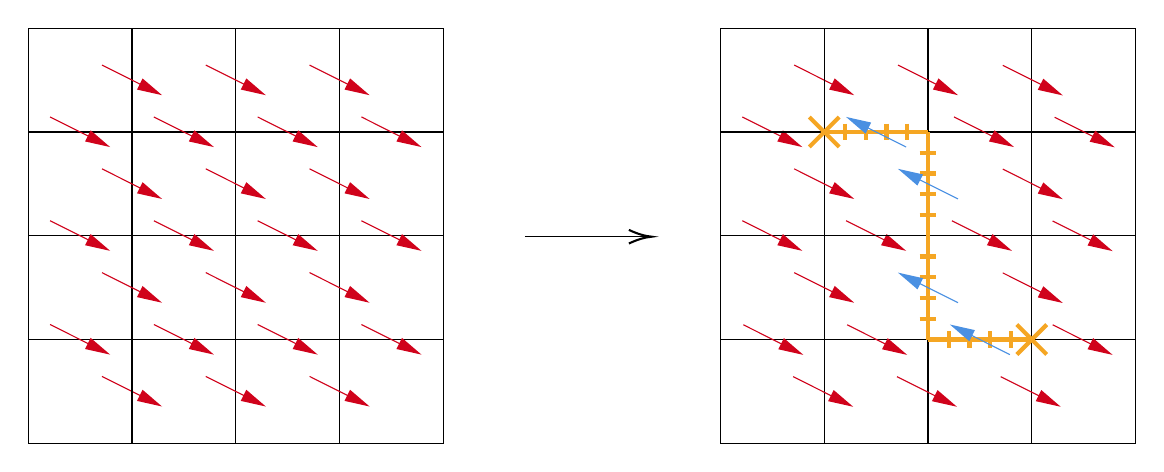
\begin{tikzpicture}[x=0.75pt,y=0.75pt,yscale=-1,xscale=1]
%uncomment if require: \path (0,300); %set diagram left start at 0, and has height of 300

%Shape: Square [id:dp3176853045406567] 
\draw   (413,192.06) -- (463,192.06) -- (463,242.06) -- (413,242.06) -- cycle ;
%Shape: Square [id:dp7022572838953951] 
\draw   (513,192.06) -- (563,192.06) -- (563,242.06) -- (513,242.06) -- cycle ;
%Shape: Square [id:dp030329102095208782] 
\draw   (513,142.06) -- (563,142.06) -- (563,192.06) -- (513,192.06) -- cycle ;
%Shape: Square [id:dp517134688980474] 
\draw   (463,192.06) -- (513,192.06) -- (513,242.06) -- (463,242.06) -- cycle ;
%Shape: Square [id:dp47682705008824966] 
\draw   (363,42.06) -- (413,42.06) -- (413,92.06) -- (363,92.06) -- cycle ;
%Shape: Square [id:dp40774233163885887] 
\draw   (413,42.06) -- (463,42.06) -- (463,92.06) -- (413,92.06) -- cycle ;
%Shape: Square [id:dp8421641317700328] 
\draw   (363,92.06) -- (413,92.06) -- (413,142.06) -- (363,142.06) -- cycle ;
%Shape: Square [id:dp8149136823625276] 
\draw   (413,92.06) -- (463,92.06) -- (463,142.06) -- (413,142.06) -- cycle ;
%Shape: Square [id:dp9420804931616191] 
\draw   (463,42.06) -- (513,42.06) -- (513,92.06) -- (463,92.06) -- cycle ;
%Shape: Square [id:dp575792276688039] 
\draw   (463,92.06) -- (513,92.06) -- (513,142.06) -- (463,142.06) -- cycle ;
%Shape: Square [id:dp604089614437928] 
\draw   (363,142.06) -- (413,142.06) -- (413,192.06) -- (363,192.06) -- cycle ;
%Shape: Square [id:dp9110252712752467] 
\draw   (413,142.06) -- (463,142.06) -- (463,192.06) -- (413,192.06) -- cycle ;
%Shape: Square [id:dp757512175683634] 
\draw   (463,142.06) -- (513,142.06) -- (513,192.06) -- (463,192.06) -- cycle ;
%Straight Lines [id:da24590588647520528] 
\draw [color={rgb, 255:red, 245; green, 166; blue, 35 }  ,draw opacity=1 ][line width=1.5]    (513,192.06) ;
\draw [shift={(513,192.06)}, rotate = 45] [color={rgb, 255:red, 245; green, 166; blue, 35 }  ,draw opacity=1 ][line width=1.5]    (-10.17,0) -- (10.17,0)(0,10.17) -- (0,-10.17)   ;
%Straight Lines [id:da734113367713265] 
\draw [color={rgb, 255:red, 245; green, 166; blue, 35 }  ,draw opacity=1 ][line width=1.5]    (463,192.06) -- (513,192.06) (473,188.06) -- (473,196.06)(483,188.06) -- (483,196.06)(493,188.06) -- (493,196.06)(503,188.06) -- (503,196.06) ;
%Straight Lines [id:da8677740521877175] 
\draw [color={rgb, 255:red, 245; green, 166; blue, 35 }  ,draw opacity=1 ][line width=1.5]    (463,192.06) -- (463,142.06) (459,182.06) -- (467,182.06)(459,172.06) -- (467,172.06)(459,162.06) -- (467,162.06)(459,152.06) -- (467,152.06) ;
%Straight Lines [id:da9217711157137525] 
\draw [color={rgb, 255:red, 208; green, 2; blue, 27 }  ,draw opacity=1 ]   (398.54,59.81) -- (425.67,73.42) ;
\draw [shift={(427.46,74.31)}, rotate = 206.63] [fill={rgb, 255:red, 208; green, 2; blue, 27 }  ,fill opacity=1 ][line width=0.08]  [draw opacity=0] (12,-3) -- (0,0) -- (12,3) -- cycle    ;
%Straight Lines [id:da8231785182807179] 
\draw    (413,42.06) -- (413,92.06) ;
%Straight Lines [id:da41308525995744727] 
\draw    (413,92.06) -- (413,142.06) ;
%Straight Lines [id:da3012120677599419] 
\draw [color={rgb, 255:red, 208; green, 2; blue, 27 }  ,draw opacity=1 ]   (373.54,84.81) -- (400.67,98.42) ;
\draw [shift={(402.46,99.31)}, rotate = 206.63] [fill={rgb, 255:red, 208; green, 2; blue, 27 }  ,fill opacity=1 ][line width=0.08]  [draw opacity=0] (12,-3) -- (0,0) -- (12,3) -- cycle    ;
%Straight Lines [id:da05997957846750057] 
\draw    (363,92.06) -- (413,92.06) ;
%Straight Lines [id:da3962017480147524] 
\draw [color={rgb, 255:red, 208; green, 2; blue, 27 }  ,draw opacity=1 ]   (398.54,109.81) -- (425.67,123.42) ;
\draw [shift={(427.46,124.31)}, rotate = 206.63] [fill={rgb, 255:red, 208; green, 2; blue, 27 }  ,fill opacity=1 ][line width=0.08]  [draw opacity=0] (12,-3) -- (0,0) -- (12,3) -- cycle    ;
%Straight Lines [id:da8887410805092772] 
\draw [color={rgb, 255:red, 74; green, 144; blue, 226 }  ,draw opacity=1 ]   (477.46,174.31) -- (450.33,160.71) ;
\draw [shift={(448.54,159.81)}, rotate = 386.63] [fill={rgb, 255:red, 74; green, 144; blue, 226 }  ,fill opacity=1 ][line width=0.08]  [draw opacity=0] (12,-3) -- (0,0) -- (12,3) -- cycle    ;
%Straight Lines [id:da3161585135502756] 
\draw [color={rgb, 255:red, 74; green, 144; blue, 226 }  ,draw opacity=1 ]   (502.46,199.31) -- (475.33,185.71) ;
\draw [shift={(473.54,184.81)}, rotate = 386.63] [fill={rgb, 255:red, 74; green, 144; blue, 226 }  ,fill opacity=1 ][line width=0.08]  [draw opacity=0] (12,-3) -- (0,0) -- (12,3) -- cycle    ;
%Straight Lines [id:da02918311398315465] 
\draw    (463,42.06) -- (463,92.06) ;
%Straight Lines [id:da2940193548924497] 
\draw [color={rgb, 255:red, 208; green, 2; blue, 27 }  ,draw opacity=1 ]   (448.54,59.81) -- (475.67,73.42) ;
\draw [shift={(477.46,74.31)}, rotate = 206.63] [fill={rgb, 255:red, 208; green, 2; blue, 27 }  ,fill opacity=1 ][line width=0.08]  [draw opacity=0] (12,-3) -- (0,0) -- (12,3) -- cycle    ;
%Straight Lines [id:da2999016051074743] 
\draw [color={rgb, 255:red, 208; green, 2; blue, 27 }  ,draw opacity=1 ]   (423.54,134.81) -- (450.67,148.42) ;
\draw [shift={(452.46,149.31)}, rotate = 206.63] [fill={rgb, 255:red, 208; green, 2; blue, 27 }  ,fill opacity=1 ][line width=0.08]  [draw opacity=0] (12,-3) -- (0,0) -- (12,3) -- cycle    ;
%Straight Lines [id:da13812102603223497] 
\draw    (413,142.06) -- (463,142.06) ;
%Straight Lines [id:da473115693085842] 
\draw [color={rgb, 255:red, 245; green, 166; blue, 35 }  ,draw opacity=1 ][line width=1.5]    (413,92.06) -- (463,92.06) (423,88.06) -- (423,96.06)(433,88.06) -- (433,96.06)(443,88.06) -- (443,96.06)(453,88.06) -- (453,96.06) ;
%Straight Lines [id:da21779160831084354] 
\draw [color={rgb, 255:red, 245; green, 166; blue, 35 }  ,draw opacity=1 ][line width=1.5]    (463,142.06) -- (463,92.06) (459,132.06) -- (467,132.06)(459,122.06) -- (467,122.06)(459,112.06) -- (467,112.06)(459,102.06) -- (467,102.06) ;
%Straight Lines [id:da08642153104428818] 
\draw    (363,142.06) -- (413,142.06) ;
%Straight Lines [id:da6951119379014274] 
\draw [color={rgb, 255:red, 208; green, 2; blue, 27 }  ,draw opacity=1 ]   (373.54,134.81) -- (400.67,148.42) ;
\draw [shift={(402.46,149.31)}, rotate = 206.63] [fill={rgb, 255:red, 208; green, 2; blue, 27 }  ,fill opacity=1 ][line width=0.08]  [draw opacity=0] (12,-3) -- (0,0) -- (12,3) -- cycle    ;
%Straight Lines [id:da08264979104155512] 
\draw    (413,142.06) -- (413,192.06) ;
%Straight Lines [id:da8129978724657629] 
\draw [color={rgb, 255:red, 208; green, 2; blue, 27 }  ,draw opacity=1 ]   (398.54,159.81) -- (425.67,173.42) ;
\draw [shift={(427.46,174.31)}, rotate = 206.63] [fill={rgb, 255:red, 208; green, 2; blue, 27 }  ,fill opacity=1 ][line width=0.08]  [draw opacity=0] (12,-3) -- (0,0) -- (12,3) -- cycle    ;
%Straight Lines [id:da16655027105891573] 
\draw [color={rgb, 255:red, 208; green, 2; blue, 27 }  ,draw opacity=1 ]   (474.54,134.81) -- (501.67,148.42) ;
\draw [shift={(503.46,149.31)}, rotate = 206.63] [fill={rgb, 255:red, 208; green, 2; blue, 27 }  ,fill opacity=1 ][line width=0.08]  [draw opacity=0] (12,-3) -- (0,0) -- (12,3) -- cycle    ;
%Straight Lines [id:da961269861360253] 
\draw [color={rgb, 255:red, 208; green, 2; blue, 27 }  ,draw opacity=1 ]   (475.54,84.81) -- (502.67,98.42) ;
\draw [shift={(504.46,99.31)}, rotate = 206.63] [fill={rgb, 255:red, 208; green, 2; blue, 27 }  ,fill opacity=1 ][line width=0.08]  [draw opacity=0] (12,-3) -- (0,0) -- (12,3) -- cycle    ;
%Straight Lines [id:da8577823672113685] 
\draw [color={rgb, 255:red, 74; green, 144; blue, 226 }  ,draw opacity=1 ]   (452.46,99.31) -- (425.33,85.71) ;
\draw [shift={(423.54,84.81)}, rotate = 386.63] [fill={rgb, 255:red, 74; green, 144; blue, 226 }  ,fill opacity=1 ][line width=0.08]  [draw opacity=0] (12,-3) -- (0,0) -- (12,3) -- cycle    ;
%Straight Lines [id:da682500900340755] 
\draw [color={rgb, 255:red, 74; green, 144; blue, 226 }  ,draw opacity=1 ]   (477.46,124.31) -- (450.33,110.71) ;
\draw [shift={(448.54,109.81)}, rotate = 386.63] [fill={rgb, 255:red, 74; green, 144; blue, 226 }  ,fill opacity=1 ][line width=0.08]  [draw opacity=0] (12,-3) -- (0,0) -- (12,3) -- cycle    ;
%Straight Lines [id:da09306781133035313] 
\draw [color={rgb, 255:red, 245; green, 166; blue, 35 }  ,draw opacity=1 ][line width=1.5]    (413,92.06) ;
\draw [shift={(413,92.06)}, rotate = 45] [color={rgb, 255:red, 245; green, 166; blue, 35 }  ,draw opacity=1 ][line width=1.5]    (-10.17,0) -- (10.17,0)(0,10.17) -- (0,-10.17)   ;

%Shape: Square [id:dp8465447023173558] 
\draw   (363,192.06) -- (413,192.06) -- (413,242.06) -- (363,242.06) -- cycle ;
%Shape: Square [id:dp9438298309585613] 
\draw   (513,42.06) -- (563,42.06) -- (563,92.06) -- (513,92.06) -- cycle ;
%Shape: Square [id:dp6994512173158287] 
\draw   (513,92.06) -- (563,92.06) -- (563,142.06) -- (513,142.06) -- cycle ;
%Straight Lines [id:da8418892124168778] 
\draw [color={rgb, 255:red, 208; green, 2; blue, 27 }  ,draw opacity=1 ]   (498.04,209.94) -- (525.17,223.54) ;
\draw [shift={(526.96,224.44)}, rotate = 206.63] [fill={rgb, 255:red, 208; green, 2; blue, 27 }  ,fill opacity=1 ][line width=0.08]  [draw opacity=0] (12,-3) -- (0,0) -- (12,3) -- cycle    ;
%Straight Lines [id:da9061042682723188] 
\draw [color={rgb, 255:red, 208; green, 2; blue, 27 }  ,draw opacity=1 ]   (448.04,209.94) -- (475.17,223.54) ;
\draw [shift={(476.96,224.44)}, rotate = 206.63] [fill={rgb, 255:red, 208; green, 2; blue, 27 }  ,fill opacity=1 ][line width=0.08]  [draw opacity=0] (12,-3) -- (0,0) -- (12,3) -- cycle    ;
%Straight Lines [id:da7687163300487452] 
\draw [color={rgb, 255:red, 208; green, 2; blue, 27 }  ,draw opacity=1 ]   (398.04,209.94) -- (425.17,223.54) ;
\draw [shift={(426.96,224.44)}, rotate = 206.63] [fill={rgb, 255:red, 208; green, 2; blue, 27 }  ,fill opacity=1 ][line width=0.08]  [draw opacity=0] (12,-3) -- (0,0) -- (12,3) -- cycle    ;
%Straight Lines [id:da22859514957556426] 
\draw    (512.5,92.19) -- (562.5,92.19) ;
%Straight Lines [id:da8368486354382343] 
\draw [color={rgb, 255:red, 208; green, 2; blue, 27 }  ,draw opacity=1 ]   (523.04,134.94) -- (550.17,148.54) ;
\draw [shift={(551.96,149.44)}, rotate = 206.63] [fill={rgb, 255:red, 208; green, 2; blue, 27 }  ,fill opacity=1 ][line width=0.08]  [draw opacity=0] (12,-3) -- (0,0) -- (12,3) -- cycle    ;
%Straight Lines [id:da284559803269298] 
\draw [color={rgb, 255:red, 208; green, 2; blue, 27 }  ,draw opacity=1 ]   (523.04,184.94) -- (550.17,198.54) ;
\draw [shift={(551.96,199.44)}, rotate = 206.63] [fill={rgb, 255:red, 208; green, 2; blue, 27 }  ,fill opacity=1 ][line width=0.08]  [draw opacity=0] (12,-3) -- (0,0) -- (12,3) -- cycle    ;
%Straight Lines [id:da7109167776610843] 
\draw [color={rgb, 255:red, 208; green, 2; blue, 27 }  ,draw opacity=1 ]   (374.04,184.94) -- (401.17,198.54) ;
\draw [shift={(402.96,199.44)}, rotate = 206.63] [fill={rgb, 255:red, 208; green, 2; blue, 27 }  ,fill opacity=1 ][line width=0.08]  [draw opacity=0] (12,-3) -- (0,0) -- (12,3) -- cycle    ;
%Straight Lines [id:da7975065936613515] 
\draw [color={rgb, 255:red, 208; green, 2; blue, 27 }  ,draw opacity=1 ]   (524.04,84.94) -- (551.17,98.54) ;
\draw [shift={(552.96,99.44)}, rotate = 206.63] [fill={rgb, 255:red, 208; green, 2; blue, 27 }  ,fill opacity=1 ][line width=0.08]  [draw opacity=0] (12,-3) -- (0,0) -- (12,3) -- cycle    ;
%Straight Lines [id:da1414304216799871] 
\draw [color={rgb, 255:red, 208; green, 2; blue, 27 }  ,draw opacity=1 ]   (424.04,184.94) -- (451.17,198.54) ;
\draw [shift={(452.96,199.44)}, rotate = 206.63] [fill={rgb, 255:red, 208; green, 2; blue, 27 }  ,fill opacity=1 ][line width=0.08]  [draw opacity=0] (12,-3) -- (0,0) -- (12,3) -- cycle    ;
%Straight Lines [id:da0049146308443612785] 
\draw [color={rgb, 255:red, 208; green, 2; blue, 27 }  ,draw opacity=1 ]   (499.04,109.94) -- (526.17,123.54) ;
\draw [shift={(527.96,124.44)}, rotate = 206.63] [fill={rgb, 255:red, 208; green, 2; blue, 27 }  ,fill opacity=1 ][line width=0.08]  [draw opacity=0] (12,-3) -- (0,0) -- (12,3) -- cycle    ;
%Straight Lines [id:da45851520453208705] 
\draw [color={rgb, 255:red, 208; green, 2; blue, 27 }  ,draw opacity=1 ]   (499.04,159.94) -- (526.17,173.54) ;
\draw [shift={(527.96,174.44)}, rotate = 206.63] [fill={rgb, 255:red, 208; green, 2; blue, 27 }  ,fill opacity=1 ][line width=0.08]  [draw opacity=0] (12,-3) -- (0,0) -- (12,3) -- cycle    ;
%Straight Lines [id:da193368586544167] 
\draw [color={rgb, 255:red, 208; green, 2; blue, 27 }  ,draw opacity=1 ]   (499.04,59.94) -- (526.17,73.54) ;
\draw [shift={(527.96,74.44)}, rotate = 206.63] [fill={rgb, 255:red, 208; green, 2; blue, 27 }  ,fill opacity=1 ][line width=0.08]  [draw opacity=0] (12,-3) -- (0,0) -- (12,3) -- cycle    ;
%Shape: Square [id:dp2944681179982789] 
\draw   (29.5,42.06) -- (79.5,42.06) -- (79.5,92.06) -- (29.5,92.06) -- cycle ;
%Shape: Square [id:dp9907886405428181] 
\draw   (79.5,42.06) -- (129.5,42.06) -- (129.5,92.06) -- (79.5,92.06) -- cycle ;
%Shape: Square [id:dp6519502476448713] 
\draw   (29.5,92.06) -- (79.5,92.06) -- (79.5,142.06) -- (29.5,142.06) -- cycle ;
%Shape: Square [id:dp7925682746127443] 
\draw   (79.5,92.06) -- (129.5,92.06) -- (129.5,142.06) -- (79.5,142.06) -- cycle ;
%Shape: Square [id:dp5442048196323481] 
\draw   (129.5,42.06) -- (179.5,42.06) -- (179.5,92.06) -- (129.5,92.06) -- cycle ;
%Shape: Square [id:dp25248026898484044] 
\draw   (129.5,92.06) -- (179.5,92.06) -- (179.5,142.06) -- (129.5,142.06) -- cycle ;
%Shape: Square [id:dp7775590480268038] 
\draw   (29.5,142.06) -- (79.5,142.06) -- (79.5,192.06) -- (29.5,192.06) -- cycle ;
%Shape: Square [id:dp1338343200880323] 
\draw   (79.5,142.06) -- (129.5,142.06) -- (129.5,192.06) -- (79.5,192.06) -- cycle ;
%Shape: Square [id:dp7088532821434324] 
\draw   (129.5,142.06) -- (179.5,142.06) -- (179.5,192.06) -- (129.5,192.06) -- cycle ;
%Straight Lines [id:da2700497890258473] 
\draw    (79.5,42.06) -- (79.5,92.06) ;
%Straight Lines [id:da2937434592243895] 
\draw    (79.5,92.06) -- (79.5,142.06) ;
%Straight Lines [id:da32767216765463614] 
\draw    (29.5,92.06) -- (79.5,92.06) ;
%Straight Lines [id:da2701106509000726] 
\draw    (129.5,42.06) -- (129.5,92.06) ;
%Straight Lines [id:da28944079432298353] 
\draw    (79.5,142.06) -- (129.5,142.06) ;
%Straight Lines [id:da7898411476311509] 
\draw    (29.5,142.06) -- (79.5,142.06) ;
%Straight Lines [id:da03266817725577198] 
\draw    (79.5,142.06) -- (79.5,192.06) ;
%Straight Lines [id:da8791797326384476] 
\draw [color={rgb, 255:red, 208; green, 2; blue, 27 }  ,draw opacity=1 ]   (65.04,59.81) -- (92.17,73.42) ;
\draw [shift={(93.96,74.31)}, rotate = 206.63] [fill={rgb, 255:red, 208; green, 2; blue, 27 }  ,fill opacity=1 ][line width=0.08]  [draw opacity=0] (12,-3) -- (0,0) -- (12,3) -- cycle    ;
%Straight Lines [id:da14031419653980737] 
\draw    (129.5,92.06) -- (129.5,142.06) ;
%Straight Lines [id:da5977365206916692] 
\draw    (129.5,142.06) -- (129.5,192.06) ;
%Straight Lines [id:da9839694802864396] 
\draw    (129.5,92.06) -- (179.5,92.06) ;
%Straight Lines [id:da018334436378720564] 
\draw    (129.5,142.06) -- (179.5,142.06) ;
%Straight Lines [id:da09894691687093027] 
\draw    (79.5,92.06) -- (129.5,92.06) ;
%Straight Lines [id:da9778402930655135] 
\draw [color={rgb, 255:red, 208; green, 2; blue, 27 }  ,draw opacity=1 ]   (115.04,59.81) -- (142.17,73.42) ;
\draw [shift={(143.96,74.31)}, rotate = 206.63] [fill={rgb, 255:red, 208; green, 2; blue, 27 }  ,fill opacity=1 ][line width=0.08]  [draw opacity=0] (12,-3) -- (0,0) -- (12,3) -- cycle    ;
%Straight Lines [id:da13706788423900362] 
\draw [color={rgb, 255:red, 208; green, 2; blue, 27 }  ,draw opacity=1 ]   (90.04,84.81) -- (117.17,98.42) ;
\draw [shift={(118.96,99.31)}, rotate = 206.63] [fill={rgb, 255:red, 208; green, 2; blue, 27 }  ,fill opacity=1 ][line width=0.08]  [draw opacity=0] (12,-3) -- (0,0) -- (12,3) -- cycle    ;
%Straight Lines [id:da07422420860788348] 
\draw [color={rgb, 255:red, 208; green, 2; blue, 27 }  ,draw opacity=1 ]   (40.04,84.81) -- (67.17,98.42) ;
\draw [shift={(68.96,99.31)}, rotate = 206.63] [fill={rgb, 255:red, 208; green, 2; blue, 27 }  ,fill opacity=1 ][line width=0.08]  [draw opacity=0] (12,-3) -- (0,0) -- (12,3) -- cycle    ;
%Straight Lines [id:da266151243916958] 
\draw [color={rgb, 255:red, 208; green, 2; blue, 27 }  ,draw opacity=1 ]   (140.04,84.81) -- (167.17,98.42) ;
\draw [shift={(168.96,99.31)}, rotate = 206.63] [fill={rgb, 255:red, 208; green, 2; blue, 27 }  ,fill opacity=1 ][line width=0.08]  [draw opacity=0] (12,-3) -- (0,0) -- (12,3) -- cycle    ;
%Straight Lines [id:da7305761483239985] 
\draw [color={rgb, 255:red, 208; green, 2; blue, 27 }  ,draw opacity=1 ]   (65.04,109.81) -- (92.17,123.42) ;
\draw [shift={(93.96,124.31)}, rotate = 206.63] [fill={rgb, 255:red, 208; green, 2; blue, 27 }  ,fill opacity=1 ][line width=0.08]  [draw opacity=0] (12,-3) -- (0,0) -- (12,3) -- cycle    ;
%Straight Lines [id:da26390191757327797] 
\draw [color={rgb, 255:red, 208; green, 2; blue, 27 }  ,draw opacity=1 ]   (115.04,109.81) -- (142.17,123.42) ;
\draw [shift={(143.96,124.31)}, rotate = 206.63] [fill={rgb, 255:red, 208; green, 2; blue, 27 }  ,fill opacity=1 ][line width=0.08]  [draw opacity=0] (12,-3) -- (0,0) -- (12,3) -- cycle    ;
%Straight Lines [id:da39405663144228087] 
\draw [color={rgb, 255:red, 208; green, 2; blue, 27 }  ,draw opacity=1 ]   (90.04,134.81) -- (117.17,148.42) ;
\draw [shift={(118.96,149.31)}, rotate = 206.63] [fill={rgb, 255:red, 208; green, 2; blue, 27 }  ,fill opacity=1 ][line width=0.08]  [draw opacity=0] (12,-3) -- (0,0) -- (12,3) -- cycle    ;
%Straight Lines [id:da4635634803052915] 
\draw [color={rgb, 255:red, 208; green, 2; blue, 27 }  ,draw opacity=1 ]   (140.04,134.81) -- (167.17,148.42) ;
\draw [shift={(168.96,149.31)}, rotate = 206.63] [fill={rgb, 255:red, 208; green, 2; blue, 27 }  ,fill opacity=1 ][line width=0.08]  [draw opacity=0] (12,-3) -- (0,0) -- (12,3) -- cycle    ;
%Straight Lines [id:da5943890262371219] 
\draw [color={rgb, 255:red, 208; green, 2; blue, 27 }  ,draw opacity=1 ]   (40.04,134.81) -- (67.17,148.42) ;
\draw [shift={(68.96,149.31)}, rotate = 206.63] [fill={rgb, 255:red, 208; green, 2; blue, 27 }  ,fill opacity=1 ][line width=0.08]  [draw opacity=0] (12,-3) -- (0,0) -- (12,3) -- cycle    ;
%Straight Lines [id:da6028394051065804] 
\draw [color={rgb, 255:red, 208; green, 2; blue, 27 }  ,draw opacity=1 ]   (65.04,159.81) -- (92.17,173.42) ;
\draw [shift={(93.96,174.31)}, rotate = 206.63] [fill={rgb, 255:red, 208; green, 2; blue, 27 }  ,fill opacity=1 ][line width=0.08]  [draw opacity=0] (12,-3) -- (0,0) -- (12,3) -- cycle    ;
%Straight Lines [id:da507884443037212] 
\draw [color={rgb, 255:red, 208; green, 2; blue, 27 }  ,draw opacity=1 ]   (115.04,159.81) -- (142.17,173.42) ;
\draw [shift={(143.96,174.31)}, rotate = 206.63] [fill={rgb, 255:red, 208; green, 2; blue, 27 }  ,fill opacity=1 ][line width=0.08]  [draw opacity=0] (12,-3) -- (0,0) -- (12,3) -- cycle    ;
%Straight Lines [id:da23526586798373939] 
\draw    (179.5,42.06) -- (179.5,92.06) ;
%Shape: Square [id:dp6143206523167073] 
\draw   (179.5,92.06) -- (229.5,92.06) -- (229.5,142.06) -- (179.5,142.06) -- cycle ;
%Shape: Square [id:dp0985246562755] 
\draw   (179.5,142.06) -- (229.5,142.06) -- (229.5,192.06) -- (179.5,192.06) -- cycle ;
%Shape: Square [id:dp6484371579778048] 
\draw   (179.5,42.06) -- (229.5,42.06) -- (229.5,92.06) -- (179.5,92.06) -- cycle ;
%Shape: Square [id:dp8586906674689465] 
\draw   (29.5,192.06) -- (79.5,192.06) -- (79.5,242.06) -- (29.5,242.06) -- cycle ;
%Shape: Square [id:dp04872184355539333] 
\draw   (79.5,192.06) -- (129.5,192.06) -- (129.5,242.06) -- (79.5,242.06) -- cycle ;
%Shape: Square [id:dp3103882786233412] 
\draw   (129.5,192.06) -- (179.5,192.06) -- (179.5,242.06) -- (129.5,242.06) -- cycle ;
%Shape: Square [id:dp0013830975332691509] 
\draw   (179.5,192.06) -- (229.5,192.06) -- (229.5,242.06) -- (179.5,242.06) -- cycle ;
%Straight Lines [id:da014561450380517149] 
\draw [color={rgb, 255:red, 208; green, 2; blue, 27 }  ,draw opacity=1 ]   (165.04,59.81) -- (192.17,73.42) ;
\draw [shift={(193.96,74.31)}, rotate = 206.63] [fill={rgb, 255:red, 208; green, 2; blue, 27 }  ,fill opacity=1 ][line width=0.08]  [draw opacity=0] (12,-3) -- (0,0) -- (12,3) -- cycle    ;
%Straight Lines [id:da8815895180727022] 
\draw    (179.5,92.06) -- (179.5,142.06) ;
%Straight Lines [id:da8964099918644335] 
\draw    (179.5,142.06) -- (179.5,192.06) ;
%Straight Lines [id:da7565582718111021] 
\draw    (179.5,192.06) -- (179.5,242.06) ;
%Straight Lines [id:da803623427369047] 
\draw    (129.5,192.06) -- (129.5,242.06) ;
%Straight Lines [id:da11895860097793509] 
\draw    (79.5,192.06) -- (79.5,242.06) ;
%Straight Lines [id:da05456314898380055] 
\draw [color={rgb, 255:red, 208; green, 2; blue, 27 }  ,draw opacity=1 ]   (165.04,109.81) -- (192.17,123.42) ;
\draw [shift={(193.96,124.31)}, rotate = 206.63] [fill={rgb, 255:red, 208; green, 2; blue, 27 }  ,fill opacity=1 ][line width=0.08]  [draw opacity=0] (12,-3) -- (0,0) -- (12,3) -- cycle    ;
%Straight Lines [id:da08984875889216193] 
\draw [color={rgb, 255:red, 208; green, 2; blue, 27 }  ,draw opacity=1 ]   (165.04,159.81) -- (192.17,173.42) ;
\draw [shift={(193.96,174.31)}, rotate = 206.63] [fill={rgb, 255:red, 208; green, 2; blue, 27 }  ,fill opacity=1 ][line width=0.08]  [draw opacity=0] (12,-3) -- (0,0) -- (12,3) -- cycle    ;
%Straight Lines [id:da6784600873216933] 
\draw [color={rgb, 255:red, 208; green, 2; blue, 27 }  ,draw opacity=1 ]   (165.04,209.81) -- (192.17,223.42) ;
\draw [shift={(193.96,224.31)}, rotate = 206.63] [fill={rgb, 255:red, 208; green, 2; blue, 27 }  ,fill opacity=1 ][line width=0.08]  [draw opacity=0] (12,-3) -- (0,0) -- (12,3) -- cycle    ;
%Straight Lines [id:da8487115371584568] 
\draw [color={rgb, 255:red, 208; green, 2; blue, 27 }  ,draw opacity=1 ]   (115.04,209.81) -- (142.17,223.42) ;
\draw [shift={(143.96,224.31)}, rotate = 206.63] [fill={rgb, 255:red, 208; green, 2; blue, 27 }  ,fill opacity=1 ][line width=0.08]  [draw opacity=0] (12,-3) -- (0,0) -- (12,3) -- cycle    ;
%Straight Lines [id:da9939290930501483] 
\draw [color={rgb, 255:red, 208; green, 2; blue, 27 }  ,draw opacity=1 ]   (65.04,209.81) -- (92.17,223.42) ;
\draw [shift={(93.96,224.31)}, rotate = 206.63] [fill={rgb, 255:red, 208; green, 2; blue, 27 }  ,fill opacity=1 ][line width=0.08]  [draw opacity=0] (12,-3) -- (0,0) -- (12,3) -- cycle    ;
%Straight Lines [id:da8839808429975873] 
\draw    (79.5,192.06) -- (79.5,242.06) ;
%Straight Lines [id:da1812289236897746] 
\draw    (29.5,192.06) -- (79.5,192.06) ;
%Straight Lines [id:da040898188258963186] 
\draw    (179.5,92.06) -- (229.5,92.06) ;
%Straight Lines [id:da14970457661241787] 
\draw    (179.5,142.06) -- (229.5,142.06) ;
%Straight Lines [id:da7190142368090202] 
\draw    (179.5,192.06) -- (229.5,192.06) ;
%Straight Lines [id:da10931629209917415] 
\draw [color={rgb, 255:red, 208; green, 2; blue, 27 }  ,draw opacity=1 ]   (40.04,184.81) -- (67.17,198.42) ;
\draw [shift={(68.96,199.31)}, rotate = 206.63] [fill={rgb, 255:red, 208; green, 2; blue, 27 }  ,fill opacity=1 ][line width=0.08]  [draw opacity=0] (12,-3) -- (0,0) -- (12,3) -- cycle    ;
%Straight Lines [id:da5189764682263813] 
\draw [color={rgb, 255:red, 208; green, 2; blue, 27 }  ,draw opacity=1 ]   (190.04,84.81) -- (217.17,98.42) ;
\draw [shift={(218.96,99.31)}, rotate = 206.63] [fill={rgb, 255:red, 208; green, 2; blue, 27 }  ,fill opacity=1 ][line width=0.08]  [draw opacity=0] (12,-3) -- (0,0) -- (12,3) -- cycle    ;
%Straight Lines [id:da011081053849876676] 
\draw [color={rgb, 255:red, 208; green, 2; blue, 27 }  ,draw opacity=1 ]   (190.04,134.81) -- (217.17,148.42) ;
\draw [shift={(218.96,149.31)}, rotate = 206.63] [fill={rgb, 255:red, 208; green, 2; blue, 27 }  ,fill opacity=1 ][line width=0.08]  [draw opacity=0] (12,-3) -- (0,0) -- (12,3) -- cycle    ;
%Straight Lines [id:da7442504430853205] 
\draw [color={rgb, 255:red, 208; green, 2; blue, 27 }  ,draw opacity=1 ]   (190.04,184.81) -- (217.17,198.42) ;
\draw [shift={(218.96,199.31)}, rotate = 206.63] [fill={rgb, 255:red, 208; green, 2; blue, 27 }  ,fill opacity=1 ][line width=0.08]  [draw opacity=0] (12,-3) -- (0,0) -- (12,3) -- cycle    ;
%Straight Lines [id:da3970407070395152] 
\draw    (79.5,192.06) -- (129.5,192.06) ;
%Straight Lines [id:da6055180132972338] 
\draw    (129.5,192.06) -- (179.5,192.06) ;
%Straight Lines [id:da6938740383021329] 
\draw [color={rgb, 255:red, 208; green, 2; blue, 27 }  ,draw opacity=1 ]   (140.04,184.81) -- (167.17,198.42) ;
\draw [shift={(168.96,199.31)}, rotate = 206.63] [fill={rgb, 255:red, 208; green, 2; blue, 27 }  ,fill opacity=1 ][line width=0.08]  [draw opacity=0] (12,-3) -- (0,0) -- (12,3) -- cycle    ;
%Straight Lines [id:da3372631654864733] 
\draw [color={rgb, 255:red, 208; green, 2; blue, 27 }  ,draw opacity=1 ]   (90.04,184.81) -- (117.17,198.42) ;
\draw [shift={(118.96,199.31)}, rotate = 206.63] [fill={rgb, 255:red, 208; green, 2; blue, 27 }  ,fill opacity=1 ][line width=0.08]  [draw opacity=0] (12,-3) -- (0,0) -- (12,3) -- cycle    ;

%Straight Lines [id:da2663235352080846] 
\draw    (268.83,142.5) -- (327.83,142.5) ;
\draw [shift={(329.83,142.5)}, rotate = 180] [color={rgb, 255:red, 0; green, 0; blue, 0 }  ][line width=0.75]    (10.93,-3.29) .. controls (6.95,-1.4) and (3.31,-0.3) .. (0,0) .. controls (3.31,0.3) and (6.95,1.4) .. (10.93,3.29)   ;




\end{tikzpicture}

    }
    \subfigure[将一个$O_\text{e}$开弦算符作用在已有元激发的态上得到的结果;弦开头处的e激发被运送到了弦末尾,弦上其它各点上如果原本没有e激发,那么还是没有,如果原本有,那么现在还是有]{
        

\tikzset{every picture/.style={line width=0.75pt}} %set default line width to 0.75pt        

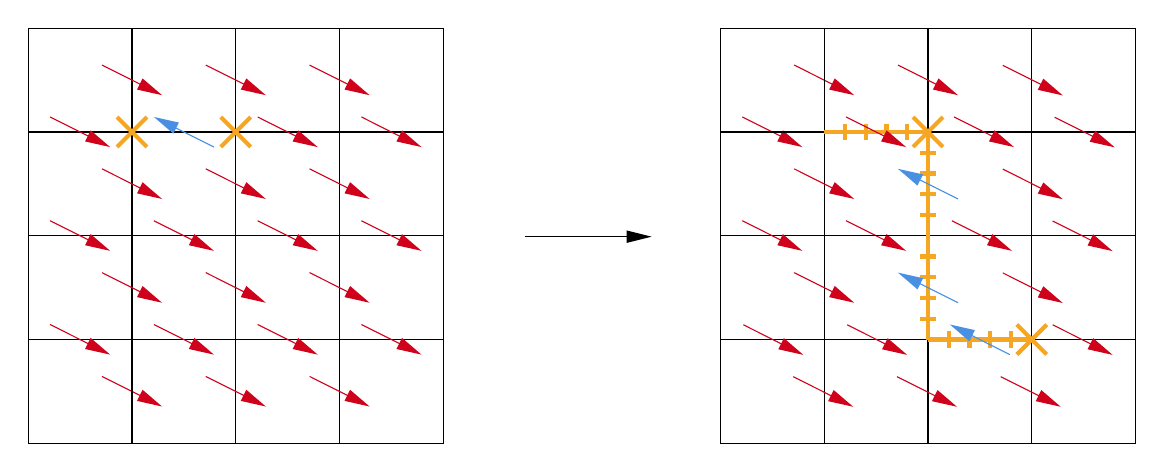
\begin{tikzpicture}[x=0.75pt,y=0.75pt,yscale=-1,xscale=1]
%uncomment if require: \path (0,300); %set diagram left start at 0, and has height of 300

%Shape: Square [id:dp36196949269788203] 
\draw   (433,212.06) -- (483,212.06) -- (483,262.06) -- (433,262.06) -- cycle ;
%Shape: Square [id:dp4539886973873315] 
\draw   (533,212.06) -- (583,212.06) -- (583,262.06) -- (533,262.06) -- cycle ;
%Shape: Square [id:dp6375978130473219] 
\draw   (533,162.06) -- (583,162.06) -- (583,212.06) -- (533,212.06) -- cycle ;
%Shape: Square [id:dp5485656687226403] 
\draw   (483,212.06) -- (533,212.06) -- (533,262.06) -- (483,262.06) -- cycle ;
%Shape: Square [id:dp7861946257195895] 
\draw   (383,62.06) -- (433,62.06) -- (433,112.06) -- (383,112.06) -- cycle ;
%Shape: Square [id:dp4265689791603251] 
\draw   (433,62.06) -- (483,62.06) -- (483,112.06) -- (433,112.06) -- cycle ;
%Shape: Square [id:dp85770876091055] 
\draw   (383,112.06) -- (433,112.06) -- (433,162.06) -- (383,162.06) -- cycle ;
%Shape: Square [id:dp9994589809447718] 
\draw   (433,112.06) -- (483,112.06) -- (483,162.06) -- (433,162.06) -- cycle ;
%Shape: Square [id:dp3934144084207285] 
\draw   (483,62.06) -- (533,62.06) -- (533,112.06) -- (483,112.06) -- cycle ;
%Shape: Square [id:dp44660161866059256] 
\draw   (483,112.06) -- (533,112.06) -- (533,162.06) -- (483,162.06) -- cycle ;
%Shape: Square [id:dp8655676597107462] 
\draw   (383,162.06) -- (433,162.06) -- (433,212.06) -- (383,212.06) -- cycle ;
%Shape: Square [id:dp31081007435708097] 
\draw   (433,162.06) -- (483,162.06) -- (483,212.06) -- (433,212.06) -- cycle ;
%Shape: Square [id:dp8086659149268767] 
\draw   (483,162.06) -- (533,162.06) -- (533,212.06) -- (483,212.06) -- cycle ;
%Straight Lines [id:da053200549000906205] 
\draw [color={rgb, 255:red, 245; green, 166; blue, 35 }  ,draw opacity=1 ][line width=1.5]    (533,212.06) ;
\draw [shift={(533,212.06)}, rotate = 45] [color={rgb, 255:red, 245; green, 166; blue, 35 }  ,draw opacity=1 ][line width=1.5]    (-10.17,0) -- (10.17,0)(0,10.17) -- (0,-10.17)   ;
%Straight Lines [id:da3649892359785114] 
\draw [color={rgb, 255:red, 245; green, 166; blue, 35 }  ,draw opacity=1 ][line width=1.5]    (483,212.06) -- (533,212.06) (493,208.06) -- (493,216.06)(503,208.06) -- (503,216.06)(513,208.06) -- (513,216.06)(523,208.06) -- (523,216.06) ;
%Straight Lines [id:da13469057648466287] 
\draw [color={rgb, 255:red, 245; green, 166; blue, 35 }  ,draw opacity=1 ][line width=1.5]    (483,212.06) -- (483,162.06) (479,202.06) -- (487,202.06)(479,192.06) -- (487,192.06)(479,182.06) -- (487,182.06)(479,172.06) -- (487,172.06) ;
%Straight Lines [id:da6345763045380002] 
\draw [color={rgb, 255:red, 208; green, 2; blue, 27 }  ,draw opacity=1 ]   (418.54,79.81) -- (445.67,93.42) ;
\draw [shift={(447.46,94.31)}, rotate = 206.63] [fill={rgb, 255:red, 208; green, 2; blue, 27 }  ,fill opacity=1 ][line width=0.08]  [draw opacity=0] (12,-3) -- (0,0) -- (12,3) -- cycle    ;
%Straight Lines [id:da5007686616056861] 
\draw    (433,62.06) -- (433,112.06) ;
%Straight Lines [id:da49682550012597915] 
\draw    (433,112.06) -- (433,162.06) ;
%Straight Lines [id:da9160145620735776] 
\draw [color={rgb, 255:red, 208; green, 2; blue, 27 }  ,draw opacity=1 ]   (393.54,104.81) -- (420.67,118.42) ;
\draw [shift={(422.46,119.31)}, rotate = 206.63] [fill={rgb, 255:red, 208; green, 2; blue, 27 }  ,fill opacity=1 ][line width=0.08]  [draw opacity=0] (12,-3) -- (0,0) -- (12,3) -- cycle    ;
%Straight Lines [id:da6394802587540938] 
\draw    (383,112.06) -- (433,112.06) ;
%Straight Lines [id:da32113469950640705] 
\draw [color={rgb, 255:red, 208; green, 2; blue, 27 }  ,draw opacity=1 ]   (418.54,129.81) -- (445.67,143.42) ;
\draw [shift={(447.46,144.31)}, rotate = 206.63] [fill={rgb, 255:red, 208; green, 2; blue, 27 }  ,fill opacity=1 ][line width=0.08]  [draw opacity=0] (12,-3) -- (0,0) -- (12,3) -- cycle    ;
%Straight Lines [id:da24099776716939703] 
\draw [color={rgb, 255:red, 74; green, 144; blue, 226 }  ,draw opacity=1 ]   (497.46,194.31) -- (470.33,180.71) ;
\draw [shift={(468.54,179.81)}, rotate = 386.63] [fill={rgb, 255:red, 74; green, 144; blue, 226 }  ,fill opacity=1 ][line width=0.08]  [draw opacity=0] (12,-3) -- (0,0) -- (12,3) -- cycle    ;
%Straight Lines [id:da5688629141790045] 
\draw [color={rgb, 255:red, 74; green, 144; blue, 226 }  ,draw opacity=1 ]   (522.46,219.31) -- (495.33,205.71) ;
\draw [shift={(493.54,204.81)}, rotate = 386.63] [fill={rgb, 255:red, 74; green, 144; blue, 226 }  ,fill opacity=1 ][line width=0.08]  [draw opacity=0] (12,-3) -- (0,0) -- (12,3) -- cycle    ;
%Straight Lines [id:da06719454989257079] 
\draw    (483,62.06) -- (483,112.06) ;
%Straight Lines [id:da3658940630124152] 
\draw [color={rgb, 255:red, 208; green, 2; blue, 27 }  ,draw opacity=1 ]   (468.54,79.81) -- (495.67,93.42) ;
\draw [shift={(497.46,94.31)}, rotate = 206.63] [fill={rgb, 255:red, 208; green, 2; blue, 27 }  ,fill opacity=1 ][line width=0.08]  [draw opacity=0] (12,-3) -- (0,0) -- (12,3) -- cycle    ;
%Straight Lines [id:da9827136653687769] 
\draw [color={rgb, 255:red, 208; green, 2; blue, 27 }  ,draw opacity=1 ]   (443.54,154.81) -- (470.67,168.42) ;
\draw [shift={(472.46,169.31)}, rotate = 206.63] [fill={rgb, 255:red, 208; green, 2; blue, 27 }  ,fill opacity=1 ][line width=0.08]  [draw opacity=0] (12,-3) -- (0,0) -- (12,3) -- cycle    ;
%Straight Lines [id:da24542517630533744] 
\draw    (433,162.06) -- (483,162.06) ;
%Straight Lines [id:da675706435803094] 
\draw [color={rgb, 255:red, 245; green, 166; blue, 35 }  ,draw opacity=1 ][line width=1.5]    (433,112.06) -- (483,112.06) (443,108.06) -- (443,116.06)(453,108.06) -- (453,116.06)(463,108.06) -- (463,116.06)(473,108.06) -- (473,116.06) ;
%Straight Lines [id:da7807078761743926] 
\draw [color={rgb, 255:red, 245; green, 166; blue, 35 }  ,draw opacity=1 ][line width=1.5]    (483,162.06) -- (483,112.06) (479,152.06) -- (487,152.06)(479,142.06) -- (487,142.06)(479,132.06) -- (487,132.06)(479,122.06) -- (487,122.06) ;
%Straight Lines [id:da49273110414826204] 
\draw    (383,162.06) -- (433,162.06) ;
%Straight Lines [id:da4909188469525809] 
\draw [color={rgb, 255:red, 208; green, 2; blue, 27 }  ,draw opacity=1 ]   (393.54,154.81) -- (420.67,168.42) ;
\draw [shift={(422.46,169.31)}, rotate = 206.63] [fill={rgb, 255:red, 208; green, 2; blue, 27 }  ,fill opacity=1 ][line width=0.08]  [draw opacity=0] (12,-3) -- (0,0) -- (12,3) -- cycle    ;
%Straight Lines [id:da7732976407163501] 
\draw    (433,162.06) -- (433,212.06) ;
%Straight Lines [id:da8885840601877579] 
\draw [color={rgb, 255:red, 208; green, 2; blue, 27 }  ,draw opacity=1 ]   (418.54,179.81) -- (445.67,193.42) ;
\draw [shift={(447.46,194.31)}, rotate = 206.63] [fill={rgb, 255:red, 208; green, 2; blue, 27 }  ,fill opacity=1 ][line width=0.08]  [draw opacity=0] (12,-3) -- (0,0) -- (12,3) -- cycle    ;
%Straight Lines [id:da7563618305941129] 
\draw [color={rgb, 255:red, 208; green, 2; blue, 27 }  ,draw opacity=1 ]   (494.54,154.81) -- (521.67,168.42) ;
\draw [shift={(523.46,169.31)}, rotate = 206.63] [fill={rgb, 255:red, 208; green, 2; blue, 27 }  ,fill opacity=1 ][line width=0.08]  [draw opacity=0] (12,-3) -- (0,0) -- (12,3) -- cycle    ;
%Straight Lines [id:da8614606849485955] 
\draw [color={rgb, 255:red, 208; green, 2; blue, 27 }  ,draw opacity=1 ]   (495.54,104.81) -- (522.67,118.42) ;
\draw [shift={(524.46,119.31)}, rotate = 206.63] [fill={rgb, 255:red, 208; green, 2; blue, 27 }  ,fill opacity=1 ][line width=0.08]  [draw opacity=0] (12,-3) -- (0,0) -- (12,3) -- cycle    ;
%Straight Lines [id:da7939198814652852] 
\draw [color={rgb, 255:red, 74; green, 144; blue, 226 }  ,draw opacity=1 ]   (497.46,144.31) -- (470.33,130.71) ;
\draw [shift={(468.54,129.81)}, rotate = 386.63] [fill={rgb, 255:red, 74; green, 144; blue, 226 }  ,fill opacity=1 ][line width=0.08]  [draw opacity=0] (12,-3) -- (0,0) -- (12,3) -- cycle    ;
%Shape: Square [id:dp106338857848296] 
\draw   (383,212.06) -- (433,212.06) -- (433,262.06) -- (383,262.06) -- cycle ;
%Shape: Square [id:dp707576745510903] 
\draw   (533,62.06) -- (583,62.06) -- (583,112.06) -- (533,112.06) -- cycle ;
%Shape: Square [id:dp32996281885734047] 
\draw   (533,112.06) -- (583,112.06) -- (583,162.06) -- (533,162.06) -- cycle ;
%Straight Lines [id:da9598175384692527] 
\draw [color={rgb, 255:red, 208; green, 2; blue, 27 }  ,draw opacity=1 ]   (518.04,229.94) -- (545.17,243.54) ;
\draw [shift={(546.96,244.44)}, rotate = 206.63] [fill={rgb, 255:red, 208; green, 2; blue, 27 }  ,fill opacity=1 ][line width=0.08]  [draw opacity=0] (12,-3) -- (0,0) -- (12,3) -- cycle    ;
%Straight Lines [id:da830133254314485] 
\draw [color={rgb, 255:red, 208; green, 2; blue, 27 }  ,draw opacity=1 ]   (468.04,229.94) -- (495.17,243.54) ;
\draw [shift={(496.96,244.44)}, rotate = 206.63] [fill={rgb, 255:red, 208; green, 2; blue, 27 }  ,fill opacity=1 ][line width=0.08]  [draw opacity=0] (12,-3) -- (0,0) -- (12,3) -- cycle    ;
%Straight Lines [id:da9456594973520096] 
\draw [color={rgb, 255:red, 208; green, 2; blue, 27 }  ,draw opacity=1 ]   (418.04,229.94) -- (445.17,243.54) ;
\draw [shift={(446.96,244.44)}, rotate = 206.63] [fill={rgb, 255:red, 208; green, 2; blue, 27 }  ,fill opacity=1 ][line width=0.08]  [draw opacity=0] (12,-3) -- (0,0) -- (12,3) -- cycle    ;
%Straight Lines [id:da9286370031442577] 
\draw    (532.5,112.19) -- (582.5,112.19) ;
%Straight Lines [id:da05035735074794423] 
\draw [color={rgb, 255:red, 208; green, 2; blue, 27 }  ,draw opacity=1 ]   (543.04,154.94) -- (570.17,168.54) ;
\draw [shift={(571.96,169.44)}, rotate = 206.63] [fill={rgb, 255:red, 208; green, 2; blue, 27 }  ,fill opacity=1 ][line width=0.08]  [draw opacity=0] (12,-3) -- (0,0) -- (12,3) -- cycle    ;
%Straight Lines [id:da3083548171838988] 
\draw [color={rgb, 255:red, 208; green, 2; blue, 27 }  ,draw opacity=1 ]   (543.04,204.94) -- (570.17,218.54) ;
\draw [shift={(571.96,219.44)}, rotate = 206.63] [fill={rgb, 255:red, 208; green, 2; blue, 27 }  ,fill opacity=1 ][line width=0.08]  [draw opacity=0] (12,-3) -- (0,0) -- (12,3) -- cycle    ;
%Straight Lines [id:da8166890828993534] 
\draw [color={rgb, 255:red, 208; green, 2; blue, 27 }  ,draw opacity=1 ]   (394.04,204.94) -- (421.17,218.54) ;
\draw [shift={(422.96,219.44)}, rotate = 206.63] [fill={rgb, 255:red, 208; green, 2; blue, 27 }  ,fill opacity=1 ][line width=0.08]  [draw opacity=0] (12,-3) -- (0,0) -- (12,3) -- cycle    ;
%Straight Lines [id:da8554659211608935] 
\draw [color={rgb, 255:red, 208; green, 2; blue, 27 }  ,draw opacity=1 ]   (544.04,104.94) -- (571.17,118.54) ;
\draw [shift={(572.96,119.44)}, rotate = 206.63] [fill={rgb, 255:red, 208; green, 2; blue, 27 }  ,fill opacity=1 ][line width=0.08]  [draw opacity=0] (12,-3) -- (0,0) -- (12,3) -- cycle    ;
%Straight Lines [id:da5375248801254273] 
\draw [color={rgb, 255:red, 208; green, 2; blue, 27 }  ,draw opacity=1 ]   (444.04,204.94) -- (471.17,218.54) ;
\draw [shift={(472.96,219.44)}, rotate = 206.63] [fill={rgb, 255:red, 208; green, 2; blue, 27 }  ,fill opacity=1 ][line width=0.08]  [draw opacity=0] (12,-3) -- (0,0) -- (12,3) -- cycle    ;
%Straight Lines [id:da09821728349202297] 
\draw [color={rgb, 255:red, 208; green, 2; blue, 27 }  ,draw opacity=1 ]   (519.04,129.94) -- (546.17,143.54) ;
\draw [shift={(547.96,144.44)}, rotate = 206.63] [fill={rgb, 255:red, 208; green, 2; blue, 27 }  ,fill opacity=1 ][line width=0.08]  [draw opacity=0] (12,-3) -- (0,0) -- (12,3) -- cycle    ;
%Straight Lines [id:da9512899383990645] 
\draw [color={rgb, 255:red, 208; green, 2; blue, 27 }  ,draw opacity=1 ]   (519.04,179.94) -- (546.17,193.54) ;
\draw [shift={(547.96,194.44)}, rotate = 206.63] [fill={rgb, 255:red, 208; green, 2; blue, 27 }  ,fill opacity=1 ][line width=0.08]  [draw opacity=0] (12,-3) -- (0,0) -- (12,3) -- cycle    ;
%Straight Lines [id:da535357998535275] 
\draw [color={rgb, 255:red, 208; green, 2; blue, 27 }  ,draw opacity=1 ]   (519.04,79.94) -- (546.17,93.54) ;
\draw [shift={(547.96,94.44)}, rotate = 206.63] [fill={rgb, 255:red, 208; green, 2; blue, 27 }  ,fill opacity=1 ][line width=0.08]  [draw opacity=0] (12,-3) -- (0,0) -- (12,3) -- cycle    ;
%Shape: Square [id:dp7990222049361821] 
\draw   (49.5,62.06) -- (99.5,62.06) -- (99.5,112.06) -- (49.5,112.06) -- cycle ;
%Shape: Square [id:dp8904550552386634] 
\draw   (99.5,62.06) -- (149.5,62.06) -- (149.5,112.06) -- (99.5,112.06) -- cycle ;
%Shape: Square [id:dp5127650109295845] 
\draw   (49.5,112.06) -- (99.5,112.06) -- (99.5,162.06) -- (49.5,162.06) -- cycle ;
%Shape: Square [id:dp12849214688436494] 
\draw   (99.5,112.06) -- (149.5,112.06) -- (149.5,162.06) -- (99.5,162.06) -- cycle ;
%Shape: Square [id:dp7737277027683318] 
\draw   (149.5,62.06) -- (199.5,62.06) -- (199.5,112.06) -- (149.5,112.06) -- cycle ;
%Shape: Square [id:dp7927352395037797] 
\draw   (149.5,112.06) -- (199.5,112.06) -- (199.5,162.06) -- (149.5,162.06) -- cycle ;
%Shape: Square [id:dp5386554622216682] 
\draw   (49.5,162.06) -- (99.5,162.06) -- (99.5,212.06) -- (49.5,212.06) -- cycle ;
%Shape: Square [id:dp111010476712055] 
\draw   (99.5,162.06) -- (149.5,162.06) -- (149.5,212.06) -- (99.5,212.06) -- cycle ;
%Shape: Square [id:dp5821419956800287] 
\draw   (149.5,162.06) -- (199.5,162.06) -- (199.5,212.06) -- (149.5,212.06) -- cycle ;
%Straight Lines [id:da6903696329395099] 
\draw    (99.5,62.06) -- (99.5,112.06) ;
%Straight Lines [id:da37681750055959395] 
\draw    (99.5,112.06) -- (99.5,162.06) ;
%Straight Lines [id:da07589525156843258] 
\draw    (49.5,112.06) -- (99.5,112.06) ;
%Straight Lines [id:da8308006113905104] 
\draw    (149.5,62.06) -- (149.5,112.06) ;
%Straight Lines [id:da7674707191655699] 
\draw    (99.5,162.06) -- (149.5,162.06) ;
%Straight Lines [id:da7594879654833071] 
\draw    (49.5,162.06) -- (99.5,162.06) ;
%Straight Lines [id:da027284503407192018] 
\draw    (99.5,162.06) -- (99.5,212.06) ;
%Straight Lines [id:da4901240737698671] 
\draw [color={rgb, 255:red, 208; green, 2; blue, 27 }  ,draw opacity=1 ]   (85.04,79.81) -- (112.17,93.42) ;
\draw [shift={(113.96,94.31)}, rotate = 206.63] [fill={rgb, 255:red, 208; green, 2; blue, 27 }  ,fill opacity=1 ][line width=0.08]  [draw opacity=0] (12,-3) -- (0,0) -- (12,3) -- cycle    ;
%Straight Lines [id:da6150555493961845] 
\draw    (149.5,112.06) -- (149.5,162.06) ;
%Straight Lines [id:da8116460068940423] 
\draw    (149.5,162.06) -- (149.5,212.06) ;
%Straight Lines [id:da5488283476959541] 
\draw    (149.5,112.06) -- (199.5,112.06) ;
%Straight Lines [id:da07732657367073692] 
\draw    (149.5,162.06) -- (199.5,162.06) ;
%Straight Lines [id:da28030930112021957] 
\draw    (99.5,112.06) -- (149.5,112.06) ;
%Straight Lines [id:da033793134933984836] 
\draw [color={rgb, 255:red, 208; green, 2; blue, 27 }  ,draw opacity=1 ]   (135.04,79.81) -- (162.17,93.42) ;
\draw [shift={(163.96,94.31)}, rotate = 206.63] [fill={rgb, 255:red, 208; green, 2; blue, 27 }  ,fill opacity=1 ][line width=0.08]  [draw opacity=0] (12,-3) -- (0,0) -- (12,3) -- cycle    ;
%Straight Lines [id:da8814413169220066] 
\draw [color={rgb, 255:red, 208; green, 2; blue, 27 }  ,draw opacity=1 ]   (443.54,104.81) -- (470.67,118.42) ;
\draw [shift={(472.46,119.31)}, rotate = 206.63] [fill={rgb, 255:red, 208; green, 2; blue, 27 }  ,fill opacity=1 ][line width=0.08]  [draw opacity=0] (12,-3) -- (0,0) -- (12,3) -- cycle    ;
%Straight Lines [id:da7806079605744642] 
\draw [color={rgb, 255:red, 208; green, 2; blue, 27 }  ,draw opacity=1 ]   (60.04,104.81) -- (87.17,118.42) ;
\draw [shift={(88.96,119.31)}, rotate = 206.63] [fill={rgb, 255:red, 208; green, 2; blue, 27 }  ,fill opacity=1 ][line width=0.08]  [draw opacity=0] (12,-3) -- (0,0) -- (12,3) -- cycle    ;
%Straight Lines [id:da5754931816488336] 
\draw [color={rgb, 255:red, 208; green, 2; blue, 27 }  ,draw opacity=1 ]   (160.04,104.81) -- (187.17,118.42) ;
\draw [shift={(188.96,119.31)}, rotate = 206.63] [fill={rgb, 255:red, 208; green, 2; blue, 27 }  ,fill opacity=1 ][line width=0.08]  [draw opacity=0] (12,-3) -- (0,0) -- (12,3) -- cycle    ;
%Straight Lines [id:da5952100515604342] 
\draw [color={rgb, 255:red, 208; green, 2; blue, 27 }  ,draw opacity=1 ]   (85.04,129.81) -- (112.17,143.42) ;
\draw [shift={(113.96,144.31)}, rotate = 206.63] [fill={rgb, 255:red, 208; green, 2; blue, 27 }  ,fill opacity=1 ][line width=0.08]  [draw opacity=0] (12,-3) -- (0,0) -- (12,3) -- cycle    ;
%Straight Lines [id:da9410359840468674] 
\draw [color={rgb, 255:red, 208; green, 2; blue, 27 }  ,draw opacity=1 ]   (135.04,129.81) -- (162.17,143.42) ;
\draw [shift={(163.96,144.31)}, rotate = 206.63] [fill={rgb, 255:red, 208; green, 2; blue, 27 }  ,fill opacity=1 ][line width=0.08]  [draw opacity=0] (12,-3) -- (0,0) -- (12,3) -- cycle    ;
%Straight Lines [id:da18562201002496082] 
\draw [color={rgb, 255:red, 208; green, 2; blue, 27 }  ,draw opacity=1 ]   (110.04,154.81) -- (137.17,168.42) ;
\draw [shift={(138.96,169.31)}, rotate = 206.63] [fill={rgb, 255:red, 208; green, 2; blue, 27 }  ,fill opacity=1 ][line width=0.08]  [draw opacity=0] (12,-3) -- (0,0) -- (12,3) -- cycle    ;
%Straight Lines [id:da11755833098770019] 
\draw [color={rgb, 255:red, 208; green, 2; blue, 27 }  ,draw opacity=1 ]   (160.04,154.81) -- (187.17,168.42) ;
\draw [shift={(188.96,169.31)}, rotate = 206.63] [fill={rgb, 255:red, 208; green, 2; blue, 27 }  ,fill opacity=1 ][line width=0.08]  [draw opacity=0] (12,-3) -- (0,0) -- (12,3) -- cycle    ;
%Straight Lines [id:da25442080979156234] 
\draw [color={rgb, 255:red, 208; green, 2; blue, 27 }  ,draw opacity=1 ]   (60.04,154.81) -- (87.17,168.42) ;
\draw [shift={(88.96,169.31)}, rotate = 206.63] [fill={rgb, 255:red, 208; green, 2; blue, 27 }  ,fill opacity=1 ][line width=0.08]  [draw opacity=0] (12,-3) -- (0,0) -- (12,3) -- cycle    ;
%Straight Lines [id:da44143500096146715] 
\draw [color={rgb, 255:red, 208; green, 2; blue, 27 }  ,draw opacity=1 ]   (85.04,179.81) -- (112.17,193.42) ;
\draw [shift={(113.96,194.31)}, rotate = 206.63] [fill={rgb, 255:red, 208; green, 2; blue, 27 }  ,fill opacity=1 ][line width=0.08]  [draw opacity=0] (12,-3) -- (0,0) -- (12,3) -- cycle    ;
%Straight Lines [id:da6699778566324532] 
\draw [color={rgb, 255:red, 208; green, 2; blue, 27 }  ,draw opacity=1 ]   (135.04,179.81) -- (162.17,193.42) ;
\draw [shift={(163.96,194.31)}, rotate = 206.63] [fill={rgb, 255:red, 208; green, 2; blue, 27 }  ,fill opacity=1 ][line width=0.08]  [draw opacity=0] (12,-3) -- (0,0) -- (12,3) -- cycle    ;
%Straight Lines [id:da9200325240479144] 
\draw    (199.5,62.06) -- (199.5,112.06) ;
%Shape: Square [id:dp7328942993667524] 
\draw   (199.5,112.06) -- (249.5,112.06) -- (249.5,162.06) -- (199.5,162.06) -- cycle ;
%Shape: Square [id:dp2890961291771639] 
\draw   (199.5,162.06) -- (249.5,162.06) -- (249.5,212.06) -- (199.5,212.06) -- cycle ;
%Shape: Square [id:dp2899655977518478] 
\draw   (199.5,62.06) -- (249.5,62.06) -- (249.5,112.06) -- (199.5,112.06) -- cycle ;
%Shape: Square [id:dp04410279330347566] 
\draw   (49.5,212.06) -- (99.5,212.06) -- (99.5,262.06) -- (49.5,262.06) -- cycle ;
%Shape: Square [id:dp4328001959850347] 
\draw   (99.5,212.06) -- (149.5,212.06) -- (149.5,262.06) -- (99.5,262.06) -- cycle ;
%Shape: Square [id:dp9817380452635807] 
\draw   (149.5,212.06) -- (199.5,212.06) -- (199.5,262.06) -- (149.5,262.06) -- cycle ;
%Shape: Square [id:dp6981091681806493] 
\draw   (199.5,212.06) -- (249.5,212.06) -- (249.5,262.06) -- (199.5,262.06) -- cycle ;
%Straight Lines [id:da5538961608697273] 
\draw [color={rgb, 255:red, 208; green, 2; blue, 27 }  ,draw opacity=1 ]   (185.04,79.81) -- (212.17,93.42) ;
\draw [shift={(213.96,94.31)}, rotate = 206.63] [fill={rgb, 255:red, 208; green, 2; blue, 27 }  ,fill opacity=1 ][line width=0.08]  [draw opacity=0] (12,-3) -- (0,0) -- (12,3) -- cycle    ;
%Straight Lines [id:da8078206711036395] 
\draw    (199.5,112.06) -- (199.5,162.06) ;
%Straight Lines [id:da23005360080717563] 
\draw    (199.5,162.06) -- (199.5,212.06) ;
%Straight Lines [id:da7962686121202824] 
\draw    (199.5,212.06) -- (199.5,262.06) ;
%Straight Lines [id:da9889990147566594] 
\draw    (149.5,212.06) -- (149.5,262.06) ;
%Straight Lines [id:da7694764072279323] 
\draw    (99.5,212.06) -- (99.5,262.06) ;
%Straight Lines [id:da2376018785872358] 
\draw [color={rgb, 255:red, 208; green, 2; blue, 27 }  ,draw opacity=1 ]   (185.04,129.81) -- (212.17,143.42) ;
\draw [shift={(213.96,144.31)}, rotate = 206.63] [fill={rgb, 255:red, 208; green, 2; blue, 27 }  ,fill opacity=1 ][line width=0.08]  [draw opacity=0] (12,-3) -- (0,0) -- (12,3) -- cycle    ;
%Straight Lines [id:da5207260238843008] 
\draw [color={rgb, 255:red, 208; green, 2; blue, 27 }  ,draw opacity=1 ]   (185.04,179.81) -- (212.17,193.42) ;
\draw [shift={(213.96,194.31)}, rotate = 206.63] [fill={rgb, 255:red, 208; green, 2; blue, 27 }  ,fill opacity=1 ][line width=0.08]  [draw opacity=0] (12,-3) -- (0,0) -- (12,3) -- cycle    ;
%Straight Lines [id:da5480042946717876] 
\draw [color={rgb, 255:red, 208; green, 2; blue, 27 }  ,draw opacity=1 ]   (185.04,229.81) -- (212.17,243.42) ;
\draw [shift={(213.96,244.31)}, rotate = 206.63] [fill={rgb, 255:red, 208; green, 2; blue, 27 }  ,fill opacity=1 ][line width=0.08]  [draw opacity=0] (12,-3) -- (0,0) -- (12,3) -- cycle    ;
%Straight Lines [id:da5023843690724528] 
\draw [color={rgb, 255:red, 208; green, 2; blue, 27 }  ,draw opacity=1 ]   (135.04,229.81) -- (162.17,243.42) ;
\draw [shift={(163.96,244.31)}, rotate = 206.63] [fill={rgb, 255:red, 208; green, 2; blue, 27 }  ,fill opacity=1 ][line width=0.08]  [draw opacity=0] (12,-3) -- (0,0) -- (12,3) -- cycle    ;
%Straight Lines [id:da48659723265136146] 
\draw [color={rgb, 255:red, 208; green, 2; blue, 27 }  ,draw opacity=1 ]   (85.04,229.81) -- (112.17,243.42) ;
\draw [shift={(113.96,244.31)}, rotate = 206.63] [fill={rgb, 255:red, 208; green, 2; blue, 27 }  ,fill opacity=1 ][line width=0.08]  [draw opacity=0] (12,-3) -- (0,0) -- (12,3) -- cycle    ;
%Straight Lines [id:da08436190038107028] 
\draw    (99.5,212.06) -- (99.5,262.06) ;
%Straight Lines [id:da8238882701325334] 
\draw    (49.5,212.06) -- (99.5,212.06) ;
%Straight Lines [id:da4713034331032184] 
\draw    (199.5,112.06) -- (249.5,112.06) ;
%Straight Lines [id:da06868085071667629] 
\draw    (199.5,162.06) -- (249.5,162.06) ;
%Straight Lines [id:da5820074071163888] 
\draw    (199.5,212.06) -- (249.5,212.06) ;
%Straight Lines [id:da44314860743375517] 
\draw [color={rgb, 255:red, 208; green, 2; blue, 27 }  ,draw opacity=1 ]   (60.04,204.81) -- (87.17,218.42) ;
\draw [shift={(88.96,219.31)}, rotate = 206.63] [fill={rgb, 255:red, 208; green, 2; blue, 27 }  ,fill opacity=1 ][line width=0.08]  [draw opacity=0] (12,-3) -- (0,0) -- (12,3) -- cycle    ;
%Straight Lines [id:da059395541772979454] 
\draw [color={rgb, 255:red, 208; green, 2; blue, 27 }  ,draw opacity=1 ]   (210.04,104.81) -- (237.17,118.42) ;
\draw [shift={(238.96,119.31)}, rotate = 206.63] [fill={rgb, 255:red, 208; green, 2; blue, 27 }  ,fill opacity=1 ][line width=0.08]  [draw opacity=0] (12,-3) -- (0,0) -- (12,3) -- cycle    ;
%Straight Lines [id:da5063118933962647] 
\draw [color={rgb, 255:red, 208; green, 2; blue, 27 }  ,draw opacity=1 ]   (210.04,154.81) -- (237.17,168.42) ;
\draw [shift={(238.96,169.31)}, rotate = 206.63] [fill={rgb, 255:red, 208; green, 2; blue, 27 }  ,fill opacity=1 ][line width=0.08]  [draw opacity=0] (12,-3) -- (0,0) -- (12,3) -- cycle    ;
%Straight Lines [id:da3889893206026507] 
\draw [color={rgb, 255:red, 208; green, 2; blue, 27 }  ,draw opacity=1 ]   (210.04,204.81) -- (237.17,218.42) ;
\draw [shift={(238.96,219.31)}, rotate = 206.63] [fill={rgb, 255:red, 208; green, 2; blue, 27 }  ,fill opacity=1 ][line width=0.08]  [draw opacity=0] (12,-3) -- (0,0) -- (12,3) -- cycle    ;
%Straight Lines [id:da643594178741393] 
\draw    (99.5,212.06) -- (149.5,212.06) ;
%Straight Lines [id:da8957855859845023] 
\draw    (149.5,212.06) -- (199.5,212.06) ;
%Straight Lines [id:da6024482081021001] 
\draw [color={rgb, 255:red, 208; green, 2; blue, 27 }  ,draw opacity=1 ]   (160.04,204.81) -- (187.17,218.42) ;
\draw [shift={(188.96,219.31)}, rotate = 206.63] [fill={rgb, 255:red, 208; green, 2; blue, 27 }  ,fill opacity=1 ][line width=0.08]  [draw opacity=0] (12,-3) -- (0,0) -- (12,3) -- cycle    ;
%Straight Lines [id:da25598314352120677] 
\draw [color={rgb, 255:red, 208; green, 2; blue, 27 }  ,draw opacity=1 ]   (110.04,204.81) -- (137.17,218.42) ;
\draw [shift={(138.96,219.31)}, rotate = 206.63] [fill={rgb, 255:red, 208; green, 2; blue, 27 }  ,fill opacity=1 ][line width=0.08]  [draw opacity=0] (12,-3) -- (0,0) -- (12,3) -- cycle    ;
%Straight Lines [id:da6536230781419683] 
\draw    (288.83,162.5) -- (347.83,162.5) ;
\draw [shift={(349.83,162.5)}, rotate = 180] [fill={rgb, 255:red, 0; green, 0; blue, 0 }  ][line width=0.08]  [draw opacity=0] (12,-3) -- (0,0) -- (12,3) -- cycle    ;
%Straight Lines [id:da9507304761845745] 
\draw [color={rgb, 255:red, 74; green, 144; blue, 226 }  ,draw opacity=1 ]   (138.96,119.31) -- (111.83,105.71) ;
\draw [shift={(110.04,104.81)}, rotate = 386.63] [fill={rgb, 255:red, 74; green, 144; blue, 226 }  ,fill opacity=1 ][line width=0.08]  [draw opacity=0] (12,-3) -- (0,0) -- (12,3) -- cycle    ;
%Straight Lines [id:da5344654488798346] 
\draw [color={rgb, 255:red, 245; green, 166; blue, 35 }  ,draw opacity=1 ][line width=1.5]    (99.5,112.06) ;
\draw [shift={(99.5,112.06)}, rotate = 45] [color={rgb, 255:red, 245; green, 166; blue, 35 }  ,draw opacity=1 ][line width=1.5]    (-10.17,0) -- (10.17,0)(0,10.17) -- (0,-10.17)   ;
%Straight Lines [id:da7415055109194719] 
\draw [color={rgb, 255:red, 245; green, 166; blue, 35 }  ,draw opacity=1 ][line width=1.5]    (149.5,112.06) ;
\draw [shift={(149.5,112.06)}, rotate = 45] [color={rgb, 255:red, 245; green, 166; blue, 35 }  ,draw opacity=1 ][line width=1.5]    (-10.17,0) -- (10.17,0)(0,10.17) -- (0,-10.17)   ;
%Straight Lines [id:da6351670278271098] 
\draw [color={rgb, 255:red, 245; green, 166; blue, 35 }  ,draw opacity=1 ][line width=1.5]    (483,112.06) ;
\draw [shift={(483,112.06)}, rotate = 45] [color={rgb, 255:red, 245; green, 166; blue, 35 }  ,draw opacity=1 ][line width=1.5]    (-10.17,0) -- (10.17,0)(0,10.17) -- (0,-10.17)   ;




\end{tikzpicture}

    }
    \caption{Toric-code模型的$O_\text{e}$开弦算符}
\end{figure}

两种激发成对出现的事实意味着可以使用弦算符描述它们的产生和消灭。首先考虑由一条边连接的两个格点,这条边上的${\sigma}^z_{\vb*{i}}$算符可以将这条边上的$x$方向的自旋翻转,因此它可以做到以下三件事:
\begin{itemize}
    \item 如果两个格点上原本没有e粒子,那么在两个格点上同时产生e粒子;
    \item 如果两个格点上原本都有e粒子,那么在两个格点上同时消灭e粒子; 
    \item 如果两个格点一个有e粒子一个没有,那么该e粒子将被转移到原本没有e粒子的格点上。
\end{itemize}
这样设一系列首尾相连的边$\{\vb*{i}\}$连接了两个格点,则弦算符
\begin{equation}
    {O}_\text{e} = \prod_{\vb*{i}} {\sigma}_{\vb*{i}}^z
\end{equation}
同样可以做到以上三件事。
同样,将以上论述中的${\sigma}^z$换成${\sigma}^x$,“格点”换成“方块”,“连接两个格点的边”换成“方块共享的边”(我们可以在每个方块中间放置一个点,从而m粒子也定义在一个格点上),同样可以定义弦算符
\begin{equation}
    {O}_\text{m} = \prod_{\vb*{i}} {\sigma}_{\vb*{i}}^x.
\end{equation}
以上讨论的都是开放的弦,闭合的弦的行为需要具体分析,且对闭弦有
\begin{equation}
    {O}_\text{e} \ket{0} = {O}_\text{m} \ket{0} = \ket{0}.
\end{equation}

通过弦算符可以检查e粒子和m粒子绕对方转一圈(实际上就是使用一个闭合的弦算符作用在一个有e粒子或者m粒子的格点上),都会多出来一个$\pi$的相位,这是因为如果一个m粒子闭弦和一个e粒子开弦有单个交点,那么它们反对易(因为同一个边上的${\sigma}^x$和${\sigma}^z$反对易)。
换而言之,e粒子和m粒子均为任意子激发:这是二维的特殊现象,因为二维的环路在二维平面上它围绕的区域被挖掉一个点之后就不可缩了,因此一个粒子转一圈之后可以有一个非零相位变化。
本节涉及的激发尚为阿贝尔统计,即转一圈之后得到的量子态和转之前只差一个$U(1)$变换;还有非阿贝尔统计,即转一圈可以转移到别的量子态上。

\subsection{任意子表}

现在的问题是,环面上的Toric-code模型中最多能够弄出来多少任意子?显然e粒子和m粒子都是任意子,虽然两者自己满足玻色统计,但它们之间有一个非平凡的相位。
我们下面将以拓扑性质分类激发,即,拓扑性质相同的激发算作一种。
可以用两个量来标记一种激发的拓扑性质:设$M_{ab}$为$b$绕着$a$转一圈导致的复数因子,$\theta_a$指的是交换两个$a$导致的复数因子(或者说一个$a$绕着另一个$a$转半圈导致的复数因子)。这样,有
\begin{equation}
    \theta_\mathrm{e} = \theta_\mathrm{m} = 1, \quad M_\mathrm{em} = - 1.
\end{equation}
除了e粒子和m粒子以外肯定还有一种$\mathrm{\epsilon}$粒子,它是一个e粒子和m粒子聚合%
\footnote{所谓聚合指的是将两个激发放得尽可能近,从而得到的复合激发。e粒子和m粒子定义在不同的格点上,因此一个e粒子和一个m粒子的聚合就是在一个正方格子中央放置一个m粒子,在它的某个角上放置一个e粒子之后得到的激发,从远处看这近似于一个粒子。}%
而成的粒子,即
\begin{equation}
    \mathrm{\epsilon} = \mathrm{e} \otimes \mathrm{m}.
\end{equation}
可以容易地验证
\begin{equation}
    M_\mathrm{e\epsilon} = M_\mathrm{m\epsilon} = -1, \quad \theta_\mathrm{\epsilon} = -1.
\end{equation}
e粒子、m粒子和$\mathrm{\epsilon}$粒子这三种拓扑激发都只能成对出现。
除了这三种激发以外还有一些平凡的激发,比如声子之类,将它们全部记为$\mathbbm{1}$。

实际上,e粒子、m粒子和$\epsilon$粒子和$\mathbbm{1}$就是全部拓扑激发。
由于$\mathbbm{1}$无论如何绕圈都不会产生附加的相位,就有
\[
    \mathbbm{1} \otimes a = a.
\]
两个e粒子放在一起,得到的就是某个边上的$\sigma^x$发生了翻转,这是一个普通的激发;m粒子和$\mathrm{\epsilon}$粒子也是如此,于是
\[
    \mathrm{e} \otimes \mathrm{e} = \mathrm{m} \otimes \mathrm{m} = \mathrm{\epsilon} \otimes \mathrm{\epsilon} = \mathbbm{1}.
\]
上式实际上说明了一个非常重要的事实:封闭流形上无论有多少拓扑激发,这个态都可以通过对基态作用一些产生算符得到,或者等价地说改变基态上某些格点的值得到,那么如果将这些拓扑激发聚合到一起,得到的只是基态上局域的一些点被改变了,也即得到了一个平凡的激发。
总之,封闭流形上所有的拓扑激发聚合在一起,只会得到平凡的激发。这就从另一个角度解释了为什么非平凡的拓扑激发一定成对出现。
$\mathrm{\epsilon}$和e粒子聚合,就相当于两个e粒子先聚合得到一个平凡的激发,剩下一个m粒子,$\mathrm{\epsilon}$粒子和m粒子聚合则会留下一个e粒子和一个平凡的激发,于是
\[
    \mathrm{\epsilon} \otimes \mathrm{e} = \mathrm{m}, \quad \mathrm{\epsilon} \otimes \mathrm{m} = \mathrm{e}.
\]
因此,e粒子、m粒子和$\epsilon$粒子和$\mathbbm{1}$在聚合运算$\otimes$下是封闭的。

\subsection{四重简并和Berry相}

\begin{figure}
    \centering
    \subfigure[二维环面的同伦群是$\mathbb{Z}_2$]{
        

\tikzset{every picture/.style={line width=0.75pt}} %set default line width to 0.75pt        

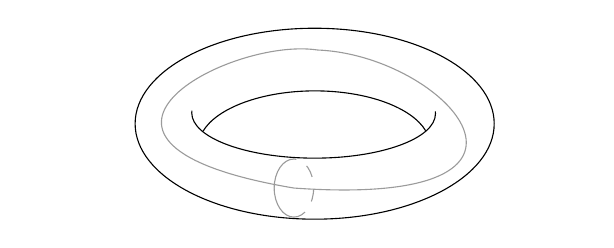
\begin{tikzpicture}[x=0.75pt,y=0.75pt,yscale=-1,xscale=1]
%uncomment if require: \path (0,300); %set diagram left start at 0, and has height of 300

%Shape: Ellipse [id:dp10888654123535657] 
\draw   (91,139) .. controls (91,113.59) and (129.73,93) .. (177.5,93) .. controls (225.27,93) and (264,113.59) .. (264,139) .. controls (264,164.41) and (225.27,185) .. (177.5,185) .. controls (129.73,185) and (91,164.41) .. (91,139) -- cycle ;
%Shape: Arc [id:dp9067895132467914] 
\draw  [draw opacity=0] (235.63,133.04) .. controls (235.69,133.42) and (235.71,133.81) .. (235.71,134.19) .. controls (235.67,146.12) and (209.35,155.7) .. (176.93,155.59) .. controls (144.5,155.48) and (118.25,145.73) .. (118.29,133.81) .. controls (118.29,133.42) and (118.32,133.05) .. (118.37,132.67) -- (177,134) -- cycle ; \draw   (235.63,133.04) .. controls (235.69,133.42) and (235.71,133.81) .. (235.71,134.19) .. controls (235.67,146.12) and (209.35,155.7) .. (176.93,155.59) .. controls (144.5,155.48) and (118.25,145.73) .. (118.29,133.81) .. controls (118.29,133.42) and (118.32,133.05) .. (118.37,132.67) ;
%Shape: Arc [id:dp7282595977083575] 
\draw  [draw opacity=0] (230.99,142.4) .. controls (224.37,131.23) and (202.8,123.1) .. (177.25,123.18) .. controls (151.77,123.27) and (130.31,131.5) .. (123.69,142.66) -- (177.34,149.79) -- cycle ; \draw   (230.99,142.4) .. controls (224.37,131.23) and (202.8,123.1) .. (177.25,123.18) .. controls (151.77,123.27) and (130.31,131.5) .. (123.69,142.66) ;

%Shape: Arc [id:dp4865327224674516] 
\draw  [draw opacity=0] (167.5,184) .. controls (167.5,184) and (167.5,184) .. (167.5,184) .. controls (162.25,184) and (158,177.73) .. (158,170) .. controls (158,162.27) and (162.25,156) .. (167.5,156) -- (167.5,170) -- cycle ; \draw  [color={rgb, 255:red, 155; green, 155; blue, 155 }  ,draw opacity=1 ] (167.5,184) .. controls (167.5,184) and (167.5,184) .. (167.5,184) .. controls (162.25,184) and (158,177.73) .. (158,170) .. controls (158,162.27) and (162.25,156) .. (167.5,156) ;
%Shape: Arc [id:dp049149640047466026] 
\draw  [draw opacity=0][dash pattern={on 4.5pt off 4.5pt}] (167.5,184) .. controls (167.5,184) and (167.5,184) .. (167.5,184) .. controls (172.75,184) and (177,177.73) .. (177,170) .. controls (177,162.27) and (172.75,156) .. (167.5,156) -- (167.5,170) -- cycle ; \draw  [color={rgb, 255:red, 155; green, 155; blue, 155 }  ,draw opacity=1 ][dash pattern={on 4.5pt off 4.5pt}] (167.5,184) .. controls (167.5,184) and (167.5,184) .. (167.5,184) .. controls (172.75,184) and (177,177.73) .. (177,170) .. controls (177,162.27) and (172.75,156) .. (167.5,156) ;

%Curve Lines [id:da7562826546508461] 
\draw [color={rgb, 255:red, 155; green, 155; blue, 155 }  ,draw opacity=1 ]   (179,103.5) .. controls (136.5,97) and (39.5,148.5) .. (167.5,170) .. controls (308,180) and (241,106) .. (179,103.5) -- cycle ;




\end{tikzpicture}
    }
    \caption{环面的拓扑性质}
\end{figure}

回忆一下,体系的希尔伯特空间维数为$2^{2N}$。当$2N-2$个边的自旋已经确定之后,系统的状态实际上已经确定了,因为约束条件\eqref{eq:toric-code-pair-condition}会确定剩下两条边的自旋。
换而言之,实际物理的希尔伯特空间维数只有$2^{2N-2}$。
这就意味着总希尔伯特空间$2^{2N}$分裂成了4支,或者说每个状态都有四重简并。
这个事实——环面上的Toric-code模型会出现基态四重简并——是\eqref{eq:toric-code-pair-condition}决定的,而\eqref{eq:toric-code-pair-condition}本身又来自环面的拓扑性质。
如果我们在哈密顿量中引入一个局部的扰动,基态能量和基态波函数显然会发生扰动,但是由于${A}$和${B}$的定义没有变化,系统拓扑没有变化,\eqref{eq:toric-code-pair-condition}也是始终成立的。
换句话说,环面上基态的四重简并是\concept{受到拓扑保护}的,局域的扰动不能让它消失。

用什么标记这四重简并?容易想到,完全可以定义一种全局性的闭弦算符,它贯穿整个环面,而由周期性边界条件它是闭弦算符。(这些算符的定义本身和拓扑紧密相关,显然如果系统被放在一个平面上那么根本没法定义全局性的闭弦算符)
分别沿着$x$轴和$y$轴定义
\begin{equation}
    {L}^x_\text{e} = \prod_{x} {\sigma}^z_{\vb*{i}}, \quad {L}^x_\text{m} = \prod_{x} {\sigma}^x_{\vb*{i}},
\end{equation}
并可以验证它们和哈密顿量是对易的,且它们构成一对对易稳定子。
这就意味着它们的本征值均为$\pm 1$,这就唯一地标记了四重简并。
以上两个弦算符显然形成了某种序,但是并不是金斯堡-朗道理论中的那种局域的序,而是一种\concept{拓扑序};相应的激发为\concept{拓扑激发}。

${L}^x_\text{e}$和${L}^x_\text{m}$将e粒子绕着$x$轴转动一圈,因此它们的本征值实际上给出了$x$方向类似于磁通量的一个通量,这个通量导致了一个Berry相位。

类似地还可以定义${L}^y_\text{e}$和${L}^y_\text{m}$,并且
\begin{equation}
    \acomm*{{L}^x_\text{e}}{{L}^y_\text{m}} = 0.
\end{equation}
我们知道
\begin{equation}
    \ket{0} = \ket{L_\text{e}^y=1, L_\text{m}^y=1},
\end{equation}
而使用这些关系可以证明,
\begin{equation}
    \begin{aligned}
        {L}^x_\text{e} \ket{0} &= \ket{L_\text{e}^y=1, L_\text{m}^y=-1}, \\
        {L}^x_\text{m} \ket{0} &= \ket{L_\text{e}^y=-1, L_\text{m}^y=1}, \\
        {L}^x_\text{m} {L}^x_\text{e} \ket{0} &= \ket{L_\text{e}^y=-1, L_\text{m}^y=-1}.
    \end{aligned}
\end{equation}
我们发现四重简并和四种基本的任意子正好能够对应上。这是拓扑序的一般特征:基态简并和任意子有对应,基态简并数目就是任意子数目的亏格次方。
我们这里是在亏格(洞的数目)为1的环面上工作,因此基态简并的数目为$4^1=4$种。
如果在亏格为0的球面上,基态简并的数目就是$4^0=1$种。
还有另一种方法也可以推导出这个结果。设亏格为$g$,由欧拉公式
\[
    V - E + F = 2 - 2g,
\]
于是
\[
    E - (V + F - 2) = 2g.
\]
而$V$是$A_s$格点的数目,$F$是$B_p$格点的数目,再减去\eqref{eq:toric-code-pair-condition}造成的两个约束,则$V+F-2$是一个二维表面Toric-code态的自由度个数。
Toric-code模型总的自由度个数为$E$,因此有$2g$个自由度用于标记简并态,由于每个自由度有两个取值,简并度为
\[
    2^{2g} = 4^g.
\]

我们看到,拓扑性质让基态简并出现,而基态简并意味着基态中可以有持续存在的弦——基态可以不是空无一物的!
这个看起来非常神奇——但是完全在预料之中——的性质让Toric-code模型成为一类允许出现弦网凝聚的模型中比较简单的一个。

\section{$\mathbb{Z}_2$规范理论}

Toric-code是一个严格可解模型;实际上,它的一些重要性质在哈密顿量形式更简单(但是不再严格可解)的所谓\concept{$\mathbb{Z}_2$规范理论}中也会体现出来。
历史上发生的事情其实是相反的:先有了$\mathbb{Z}_2$规范理论,然后再有了

\chapter{短程拓扑物态}

上一节所谓的拓扑序指的是长程的。本节是短程的,如SPT等。

\section{一维拓扑超导体}

\subsection{Kitaev链及其解析解}

以下一维模型称为\concept{Kitaev链}:
\begin{equation}
    {H} = - t \sum_{\vb*{i}} ({c}_{\vb*{i}}^\dagger {c}_{i+1} + \text{h.c.}) - \mu \sum_{\vb*{i}} {c}_{\vb*{i}}^\dagger {c}_{\vb*{i}} + \sum_{\vb*{i}} (\Delta {c}_{\vb*{i}} {c}_{i+1} + \text{h.c.} ).
    \label{eq:kitaev-chain-hamiltonian}
\end{equation}
\eqref{eq:kitaev-chain-hamiltonian}是一个p波超导模型,这个模型通常是这么来的:一个一维纳米线被放置在一个超导体上,两者的相互作用诱导前者也发生$U(1)$对称性破缺,然后我们使用平均场理论分析问题而引入一个$\Delta$参量。
\eqref{eq:kitaev-chain-hamiltonian}是一个紧束缚模型,
对\eqref{eq:kitaev-chain-hamiltonian}做傅里叶变换,可以得到
\begin{equation}
    {H} = \frac{1}{2} \sum_{\vb*{k}} \underbrace{\pmqty{{c}^\dagger_{\vb*{k}} & {c}_{-\vb*{k}}}}_{{\Psi}^\dagger} \pmqty{\epsilon_{\vb*{k}} - \mu & -2 \ii \Delta^* \sin k \\ 2 \ii \Delta \sin k & - \epsilon_{\vb*{k}} + \mu} \underbrace{\pmqty{{c}_{\vb*{k}} \\ {c}^\dagger_{-\vb*{k}}}}_{{\Psi}},
\end{equation}
然后再做Bogoliubov变换,计算出以下能谱:
\begin{equation}
    E_{\vb*{k}} = \pm \sqrt{(2t \cos k - \mu)^2 + 4 \abs{\Delta}^2 \sin^2 k}.
\end{equation}

\eqref{eq:kitaev-chain-hamiltonian}具有粒子-空穴对称性。% TODO
总之就有一个约束就是设$P$为粒子空穴变换,我们有
\[
    P {\Psi}_{\vb*{k}} P^{-1} = \tau^* {\Psi}_{-\vb*{k}}^*
\]

Kitaev链不存在对称性自发破缺,但能隙可开可闭。当
\begin{equation}
    \mu = \pm 2t
    \label{eq:kitaev-gap-point}
\end{equation}
时,能隙会关闭。除此之外任何参数的变动都只会引起连续的变化。
因此,如果体系发生相变,那么只能是在\eqref{eq:kitaev-gap-point}处发生一个和对称性无关的相变。在化学势很低时,即$\mu$趋于负无穷时,根本就没有电子,因此从$-\infty$到$-2t$的部分肯定是平庸的。
化学势非常高时(大于$2t$时)电子全满,同样是平庸的。
因此有趣的行为集中在$-2t$到$2t$之间。下面会看到,当$\mu$越过\eqref{eq:kitaev-gap-point}这两个点时,会发生一个拓扑相变。

$W = \pm 1$,这是一个定义在立体中的量?

\subsection{Kitaev链中的拓扑不变量}

下面定义一个能带的拓扑不变量。

总之,当$\mu$扫过$\mu=-2t$时,我们有
\[
    {c}_{\vb*{i}} = \frac{1}{2} ({\gamma}_{i\text{A}} + \ii {\gamma}_{i \text{B}}),
\]
容易验证均为
\begin{equation}
    \acomm*{{\gamma}_\alpha}{{\gamma}_\beta^\dagger} = 2 \delta_{\alpha \beta},
\end{equation}

\subsection{时间反演对称性保护的拓扑超导}

刚才描述的拓扑超导和对称性没有特别明确的对称性。当然可以说它有粒子-空穴对称性,但是这完全是一个数学上的处理。
